\documentclass[12pt,]{isuthesis}
\usepackage{lmodern}
\usepackage{amssymb,amsmath}
\usepackage{ifxetex,ifluatex}
\usepackage{fixltx2e} % provides \textsubscript
\ifnum 0\ifxetex 1\fi\ifluatex 1\fi=0 % if pdftex
  \usepackage[T1]{fontenc}
  \usepackage[utf8]{inputenc}
\else % if luatex or xelatex
  \ifxetex
    \usepackage{mathspec}
  \else
    \usepackage{fontspec}
  \fi
  \defaultfontfeatures{Ligatures=TeX,Scale=MatchLowercase}
\fi
% use upquote if available, for straight quotes in verbatim environments
\IfFileExists{upquote.sty}{\usepackage{upquote}}{}
% use microtype if available
\IfFileExists{microtype.sty}{%
\usepackage{microtype}
\UseMicrotypeSet[protrusion]{basicmath} % disable protrusion for tt fonts
}{}
\usepackage{hyperref}
\hypersetup{unicode=true,
            pdftitle={Interfacing R with Web Technologies for Data Acquistion and Interactive Visualization},
            pdfauthor={Carson Sievert},
            pdfborder={0 0 0},
            breaklinks=true}
\urlstyle{same}  % don't use monospace font for urls
\usepackage{color}
\usepackage{fancyvrb}
\newcommand{\VerbBar}{|}
\newcommand{\VERB}{\Verb[commandchars=\\\{\}]}
\DefineVerbatimEnvironment{Highlighting}{Verbatim}{commandchars=\\\{\}}
% Add ',fontsize=\small' for more characters per line
\usepackage{framed}
\definecolor{shadecolor}{RGB}{248,248,248}
\newenvironment{Shaded}{\begin{snugshade}}{\end{snugshade}}
\newcommand{\KeywordTok}[1]{\textcolor[rgb]{0.13,0.29,0.53}{\textbf{{#1}}}}
\newcommand{\DataTypeTok}[1]{\textcolor[rgb]{0.13,0.29,0.53}{{#1}}}
\newcommand{\DecValTok}[1]{\textcolor[rgb]{0.00,0.00,0.81}{{#1}}}
\newcommand{\BaseNTok}[1]{\textcolor[rgb]{0.00,0.00,0.81}{{#1}}}
\newcommand{\FloatTok}[1]{\textcolor[rgb]{0.00,0.00,0.81}{{#1}}}
\newcommand{\ConstantTok}[1]{\textcolor[rgb]{0.00,0.00,0.00}{{#1}}}
\newcommand{\CharTok}[1]{\textcolor[rgb]{0.31,0.60,0.02}{{#1}}}
\newcommand{\SpecialCharTok}[1]{\textcolor[rgb]{0.00,0.00,0.00}{{#1}}}
\newcommand{\StringTok}[1]{\textcolor[rgb]{0.31,0.60,0.02}{{#1}}}
\newcommand{\VerbatimStringTok}[1]{\textcolor[rgb]{0.31,0.60,0.02}{{#1}}}
\newcommand{\SpecialStringTok}[1]{\textcolor[rgb]{0.31,0.60,0.02}{{#1}}}
\newcommand{\ImportTok}[1]{{#1}}
\newcommand{\CommentTok}[1]{\textcolor[rgb]{0.56,0.35,0.01}{\textit{{#1}}}}
\newcommand{\DocumentationTok}[1]{\textcolor[rgb]{0.56,0.35,0.01}{\textbf{\textit{{#1}}}}}
\newcommand{\AnnotationTok}[1]{\textcolor[rgb]{0.56,0.35,0.01}{\textbf{\textit{{#1}}}}}
\newcommand{\CommentVarTok}[1]{\textcolor[rgb]{0.56,0.35,0.01}{\textbf{\textit{{#1}}}}}
\newcommand{\OtherTok}[1]{\textcolor[rgb]{0.56,0.35,0.01}{{#1}}}
\newcommand{\FunctionTok}[1]{\textcolor[rgb]{0.00,0.00,0.00}{{#1}}}
\newcommand{\VariableTok}[1]{\textcolor[rgb]{0.00,0.00,0.00}{{#1}}}
\newcommand{\ControlFlowTok}[1]{\textcolor[rgb]{0.13,0.29,0.53}{\textbf{{#1}}}}
\newcommand{\OperatorTok}[1]{\textcolor[rgb]{0.81,0.36,0.00}{\textbf{{#1}}}}
\newcommand{\BuiltInTok}[1]{{#1}}
\newcommand{\ExtensionTok}[1]{{#1}}
\newcommand{\PreprocessorTok}[1]{\textcolor[rgb]{0.56,0.35,0.01}{\textit{{#1}}}}
\newcommand{\AttributeTok}[1]{\textcolor[rgb]{0.77,0.63,0.00}{{#1}}}
\newcommand{\RegionMarkerTok}[1]{{#1}}
\newcommand{\InformationTok}[1]{\textcolor[rgb]{0.56,0.35,0.01}{\textbf{\textit{{#1}}}}}
\newcommand{\WarningTok}[1]{\textcolor[rgb]{0.56,0.35,0.01}{\textbf{\textit{{#1}}}}}
\newcommand{\AlertTok}[1]{\textcolor[rgb]{0.94,0.16,0.16}{{#1}}}
\newcommand{\ErrorTok}[1]{\textcolor[rgb]{0.64,0.00,0.00}{\textbf{{#1}}}}
\newcommand{\NormalTok}[1]{{#1}}
\usepackage{longtable,booktabs}

% always, graphics silly
\usepackage{graphicx,grffile}
\makeatletter
\def\maxwidth{\ifdim\Gin@nat@width>\linewidth\linewidth\else\Gin@nat@width\fi}
\def\maxheight{\ifdim\Gin@nat@height>\textheight\textheight\else\Gin@nat@height\fi}
\makeatother
% Scale images if necessary, so that they will not overflow the page
% margins by default, and it is still possible to overwrite the defaults
% using explicit options in \includegraphics[width, height, ...]{}
\setkeys{Gin}{width=\maxwidth,height=\maxheight,keepaspectratio}


\IfFileExists{parskip.sty}{%
\usepackage{parskip}
}{% else
\setlength{\parindent}{0pt}
\setlength{\parskip}{6pt plus 2pt minus 1pt}
}
\setlength{\emergencystretch}{3em}  % prevent overfull lines
\providecommand{\tightlist}{%
  \setlength{\itemsep}{0pt}\setlength{\parskip}{0pt}}
\setcounter{secnumdepth}{5}
% Redefines (sub)paragraphs to behave more like sections
\ifx\paragraph\undefined\else
\let\oldparagraph\paragraph
\renewcommand{\paragraph}[1]{\oldparagraph{#1}\mbox{}}
\fi
\ifx\subparagraph\undefined\else
\let\oldsubparagraph\subparagraph
\renewcommand{\subparagraph}[1]{\oldsubparagraph{#1}\mbox{}}
\fi

%%% Use protect on footnotes to avoid problems with footnotes in titles
\let\rmarkdownfootnote\footnote%
\def\footnote{\protect\rmarkdownfootnote}

%%% Change title format to be more compact
\usepackage{titling}

% Create subtitle command for use in maketitle
\newcommand{\subtitle}[1]{
 \posttitle{
   \begin{center}\large#1\end{center}
   }
}

\setlength{\droptitle}{-2em}
 \title{Interfacing R with Web Technologies for Data Acquistion and Interactive
Visualization}
 \pretitle{\vspace{\droptitle}\centering\huge}
 \posttitle{\par}
 \author{Carson Sievert}
 \preauthor{\centering\large\emph}
 \postauthor{\par}
 \date{}
 \predate{}\postdate{}



\begin{document}

\maketitle

{
\setcounter{tocdepth}{2}
\tableofcontents
}
\addcontentsline{toc}{chapter}{LIST OF TABLES}
\listoftables
\cleardoublepage \phantomsection \addcontentsline{toc}{chapter}{LIST OF FIGURES}
\listoffigures

\cleardoublepage \phantomsection
\specialchapt{ACKNOWLEDGEMENTS}

This thesis would not be possible without many people. First and foremost, special thanks to my major professor Heike Hofmann. I would not made it to this point without such a warm and friendly mentor who was often more confident in my abilities than I was of my own. Thank you for always supporting me no matter how many things I had going on to distract me from research. I aspire to inherit the same empathy and support that you show to your students on a daily basis. 

Another special thanks goes to Di Cook. In the fourth year of my PhD, I was experiencing burnout (and growing tired of Ames), when Di took me to lunch, told me she was transferring to Monash University in Australia, and invited me to join her. Of course, I said yes, and when I arrived, I immediately felt welcomed and a part of the group -- all thanks to Di. She strategically assigned me to assist her students with their thesis projects, run R workshops for the university, and most importantly, work on my tennis game. Through this "work" I met so many amazing people and had many memorable experiences. Those 6 months gave me a new perspective on life in general and I am forever grateful for being blessed enough to take the opportunity.

Thank you to many of Heike and Di's former students who came before me (just to name a few: Hadley Wickham, Michael Lawrence, Yihui Xie, Xiaoyue Cheng, Barrett Schloerke, Susan VanderPlas). Your work has not only inspired and enabled my work, but it has also enabled an entire community of people working with data to do amazing things. Without this strong history and community at Iowa State, I would not have had the courage or the vision to follow such a "non-traditional" research path. I hope the University continues to value this type of work as it teaches students skills that are in high demand and generally improves the way data-driven research is performed.

Thank you to all my collaborators, especially Toby Dylan Hocking. Toby and Susan VanderPlas laid the initial framework for \textbf{animint} -- which I first worked on as a Google Summer of Code student under Toby's guidance. Toby later went on write the initial version of the \texttt{ggplotly}() function in \textbf{plotly}, borrowing a lot of ideas from \textbf{animint}. As Toby became busy with other things, he introduced me to the plotly team, and eventually handed over the reigns on the project, which has helped to financially support the last year or so of grad school.

Thank you also to the plotly team, and in particular, the software engineers who work on the open source project plotly.js. My work has benefited greatly from your responsiveness to my questions, feature requests, and bug reports. I have a great amount of respect for the work that you do, and I hope this project keeps improving at its current break neck pace.

Finally, thank you to my family for their encouragement and keeping me grounded throughout this experience. Thank you to my father for the initial encouragement to pursue a PhD, conversations surrounding work-life balance, and also pushing me to "graduate before I'm 40". Thank you to my mother for her unconditional love, endless care, and predenting to understand what I do for a living. Thank you to my brothers for providing me with shelter, beer, and Twins tickets. Thank you all for your willingness to drop everything to help me at any given moment. I can't say I've always been as willing, as I have been selfish with my time during my PhD, but I hope to change that after graduation.


\newpage
\pagenumbering{arabic}
\chapter{Literature Review}

\section{What makes a good software
interface?}\label{what-makes-a-good-software-interface}

Unwin and Hofmann (Unwin and Hofmann 2009) discuss the strengths,
weaknesses, and differences between using graphical and command-line
interfaces for data analysis. Graphical user interfaces (GUIs) can be
much more intuitive to use, but at the cost of being less flexible,
precise, and repeatable. Unwin and Hofmann argue statistical software
should strive to achieve a synergy of two that leverages both of their
strengths. That is, a command-line interface when we can precisely
describe what we want and a graphical interface for ``searching for
information and interesting structures without fully specified
questions.''

Unwin and Hofmann further discuss the different audiences these
interfaces attract. Command-line interfaces typically attract ``power
users'' such as applied statisticians and statistical researchers in a
university, whereas more casual users of statistical software typically
prefer a GUI. In later sections, we discuss GUIs in greater detail
within the context of interactive statistical graphics. For now, we
briefly discuss some best practices for designing a command-line
interface for statistical computing in R.

Before authoring an interface, one should establish the target audience,
the class of problems it should address, and loosely define how the
interface should actually work. During this process, it may also be
helpful to identify your audience as being primarily composed of
\emph{software developers} or \emph{data analysts}. Developers are
typically more interested in using the interface to develop novel
software or incorporating the functionality into a larger scientific
computing environment (Jereon Ooms 2014). In this case, interactive
exploration and troubleshooting is not always a luxury, so robust
functionality is of utmost importance. On the other hand, analysts
interfaces should work well in an interactive environment since this
caters to rapid prototyping of ideas and troubleshooting of errors.

Good developer interfaces often make it easier to implement good analyst
interfaces. A great recent example of a good developer interface is the
R package \textbf{Rcpp}, which provides a seamless interface between R
with C++ (Eddelbuettel 2013). To date, more than 500 R packages use
\textbf{Rcpp} to make interfaces that are both expressive and efficient,
including the highly influential analyst interfaces such as
\textbf{tidyr} and \textbf{dplyr} (Wickham 2014); (Wickham and Francois
2014). These interfaces help analysts focus on the primary task of
wrangling data into a form suitable for visualization and statistical
modeling, rather than focusing on the implementation details behind how
the transformations are performed. (Donoho 2015) argues that these
interfaces ``May have more impact on today's practice of data analysis
than many highly-regarded theoretical statistics papers''.

Evaluating statistical computing interfaces is certainly a subjective
matter since we all have different tastes, different backgrounds, and
have different needs. It seems reasonable to evaluate an interface based
on its effectiveness and efficiency in aiding a user complete their
task, but as (Unwin and Hofmann 2009) points out, ``There is a tendency
to judge software by the most powerful tools they provide (whether with
a good interface or not)''. As a result, all too often, analysts must
spend time gaining the skills of a software developer. Good analyst
interfaces often abstract functionality from developer interfaces in a
way that allow analysts to focus on their primary task of
acquiring/analyzing/modeling/visualizing data, rather than the
implementation details. The following focuses on such work with respect
to acquiring data from the web and interactive statistical web graphics.

\section{Acquiring and wrangling web content in
R}\label{acquiring-and-wrangling-web-content-in-r}

\subsection{Interfaces for working with web
content}\label{interfaces-for-working-with-web-content}

R has a rich history of interfacing with web technologies for
accomplishing a variety of tasks such as requesting, manipulating, and
creating web content. As an important first step, extending ideas from
(Chambers 1999), Brian Ripley implemented the connections interface for
file-oriented input/output in R (Ripley 2001). This interface supports a
variety of common transfer protocols (HTTP, HTTPS, FTP), providing
access to most files on the web that can be identified with a Uniform
Resource Locator (URL). Connection objects are actually external
pointers, meaning that, instead of immediately reading the file, they
just point to the file, and make no assumptions about the actual
contents of the file.

Many functions in the base R distribution for reading data (e.g.,
\texttt{scan}, \texttt{read.table}, \texttt{read.csv}, etc.) are built
on top of connections, and provide additional functionality for parsing
well-structured plain-text into basic R data structures (vector, list,
data frame, etc.). However, the base R distribution does not provide
functionality for parsing common file formats found on the web (e.g.,
HTML, XML, JSON). In addition, the standard R connection interface
provides no support for communicating with web servers beyond a simple
HTTP GET request (Lang 2006).

The \textbf{RCurl}, \textbf{XML}, and \textbf{RJSONIO} packages were
major contributions that drastically improved our ability to request,
manipulate, and create web content from R (Nolan and Temple Lang 2014).
The \textbf{RCurl} package provides a suite of high and low level
bindings to the C library libcurl, making it possible to transfer files
over more network protocols, communicate with web servers (e.g., submit
forms, upload files, etc.), process their responses, and handle other
details such as redirects and authentication (Temple Lang 2014a). The
\textbf{XML} package provides low-level bindings to the C library
libxml2, making it possible to download, parse, manipulate, and create
XML (and HTML) (Lang 2013). To make this possible, \textbf{XML} also
provides some data structures for representing XML in R. The
\textbf{RJSONIO} package provides a mapping between R objects and
JavaScript Object Notation (JSON) (Temple Lang 2014b). These packages
were heavily used for years, but several newer interfaces have made
these tasks easier and more efficient.

The \textbf{curl}, \textbf{httr}, and \textbf{jsonlite} packages are
more modern R interfaces for requesting content on the web and
interacting with web servers. The \textbf{curl} package provides a much
simpler interface to libcurl that also supports streaming data (useful
for transferring large data), and generally has better performance than
\textbf{RCurl} (Ooms 2015). The \textbf{httr} package builds on
\textbf{curl} and organizes it's functionality around HTTP verbs (GET,
POST, etc.) (Wickham 2015a). Since most web application programming
interfaces (APIs) organize their functionality around these same verbs,
it is often very easy to write R bindings to web services with
\textbf{httr}. The \textbf{httr} package also builds on
\textbf{jsonlite} since it provides consistent mappings between R/JSON
and most most modern web APIs accept and send messages in JSON format
(Jeroen Ooms 2014a). These packages have already had a profound impact
on the investment required to interface R with web services, which are
useful for many things beyond data acquisition. For example, it is now
easy to install R packages hosted on the web (\textbf{devtools}),
perform cloud computing (\textbf{analogsea}), and archive/share
computational outputs (\textbf{dvn}, \textbf{rfigshare},
\textbf{RAmazonS3}, \textbf{googlesheets}, \textbf{rdrop2}, etc.).

The \textbf{rvest} package builds on \textbf{httr} and makes it easy to
manipulate content in HTML/XML files (Wickham 2015c). Using
\textbf{rvest} in combination with
\href{http://selectorgadget.com/}{SelectorGadget}, it is often possible
to extract structured information (e.g., tables, lists, links, etc) from
HTML with almost no knowledge/familiarity with web technologies. The
\textbf{XML2R} package has a similar goal of providing an interface to
acquire and manipulate XML content into tabular R data structures
without any working knowledge of XML/XSLT/XPath (Sievert 2014b). As a
result, these interfaces reduce the startup costs required for analysts
to acquire data from the web.

Packages such as \textbf{XML}, \textbf{XML2R}, and \textbf{rvest} can
download and parse the source of web pages, which is \emph{static}, but
extracting \emph{dynamic} web content requires additional tools. The R
package \textbf{rdom} fills this void and makes it easy to render and
access the Document Object Model (DOM) using the headless browsing
engine phantomjs (Sievert 2015a). The R package \textbf{RSelenium} can
also render dynamic web pages and simulate user actions, but its broad
scope and heavy software requirements make it harder to use and less
reliable compared to \textbf{rdom} (Harrison 2014). \textbf{rdom} is
also designed to work seamlessly with \textbf{rvest}, so that one may
use the \texttt{rdom()} function instead of \texttt{read\_html()} to
render, parse, and return the DOM as HTML (instead of just the HTML page
source).

Any combination of these R packages may be useful in acquiring data for
personal use and/or providing a higher-level interface to specific data
source(s) to increase their accessibility. The next section focuses on
such interfaces.

\subsection{Interfaces for acquiring data on the
web}\label{interfaces-for-acquiring-data-on-the-web}

The web provides access to the world's largest repository of publicly
available information and data. This provides a nice \emph{potential}
resource both teaching and practicing applied statistics, but to be
practical useful, it often requires a custom interface to make data more
accessible. If publishers follow best practices, a custom interface to
the data source usually is not needed, but this is rarely the case. Many
times structured data is embedded within larger unstructured documents,
making it difficult to incorporate into a data analysis workflow. This
is especially true of data used to inform downstream web applications,
typically in XML and/or JSON format. There are two main ways to make
such data more accessible: (1) package, document, and distribute the
data itself (2) provide functionality to acquire the data.

If the data source is fairly small, somewhat static, and freely
available with an open license, then we can directly provide data via R
packaging mechanism. In this case, it is best practice for package
authors include scripts used to acquire, transform, and clean the data.
This model is especially nice for both teaching and providing examples,
since users can easily access data by installing the R package. (Wickham
2015b) provides a nice section outlining the details of bundling data
with R packages.\footnote{This section is freely available online
  \url{http://r-pkgs.had.co.nz/data.html}.}

R packages that just provide functionality to acquire data can be more
desirable than bundling it for several reasons. In some cases, it helps
avoid legal issues with rehosting copyrighted data. Furthermore, the
source code of R packages can always be inspected, so users can verify
the cleaning and transformations performed on the data to ensure its
integrity, and suggest changes if necessary. They are also versioned,
which makes the data acquisition, and thus any downstream analysis, more
reproducible and transparent. It is also possible to handle dynamic data
with such interfaces, meaning that new data can be acquired without any
change to the underlying source code. As explained in
\protect\hyperlink{taming-pitchfx-data-with-xml2r-and-pitchrx}{Taming
PITCHf/x Data with XML2R and pitchRx}, this is an important quality of
the \textbf{pitchRx} R package since new PITCHf/x data is made available
on a daily basis.

Perhaps the largest centralized effort in this domain is lead by
\href{https://ropensci.org}{rOpenSci}, a community of R developers that,
at the time of writing, maintains more than 50 packages providing access
to scientific data ranging from bird sightings, species occurrence, and
even text/metadata from academic publications. This provides a
tremendous service to researchers who want to spend their time building
models and deriving insights from data, rather than learning the
programming skills necessary to acquire and clean it.

It's becoming increasingly clear that ``meta'' packages that standardize
the interface to data acquisition/curation in a particular domain would
be tremendously useful. However, it is not clear how such interfaces
should be designed. The R package \textbf{etl} is one step in this
direction and aims to provide a standardized interface for \emph{any}
data access package that fits into an Extract-Transform-Load paradigm
(Baumer and Sievert, n.d.). The package provides generic
\texttt{extract}-\texttt{transform}-\texttt{load} functions, but
requires package authors to write custom
\texttt{extract}-\texttt{transform} methods for the specific data
source. In theory, the default \texttt{load} method works for any
application; as well as other database management operations such as
\texttt{update} and \texttt{clean}.

\section{Dynamic interactive statistical web
graphics}\label{dynamic-interactive-statistical-web-graphics}

\subsection{Why interactive?}\label{why-interactive}

Unlike computer graphics which focuses on representing reality,
virtually; data visualization is about garnering abstract relationships
between multiple variables from visual representation. The
dimensionality of data, the number of variables can be anything, usually
more than 3D, which summons a need to get beyond 2D canvasses for
display. Technology enables this, enabling the user to see many views,
query and link components. As demonstrated in Figure \ref{fig:tour}
using the R package \textbf{tourbrush} (Sievert 2015b), interactive and
dynamic graphics allow us to go beyond the constraints of
low-dimensional displays to see high-dimensional relationships in data.

\begin{figure}

{\centering 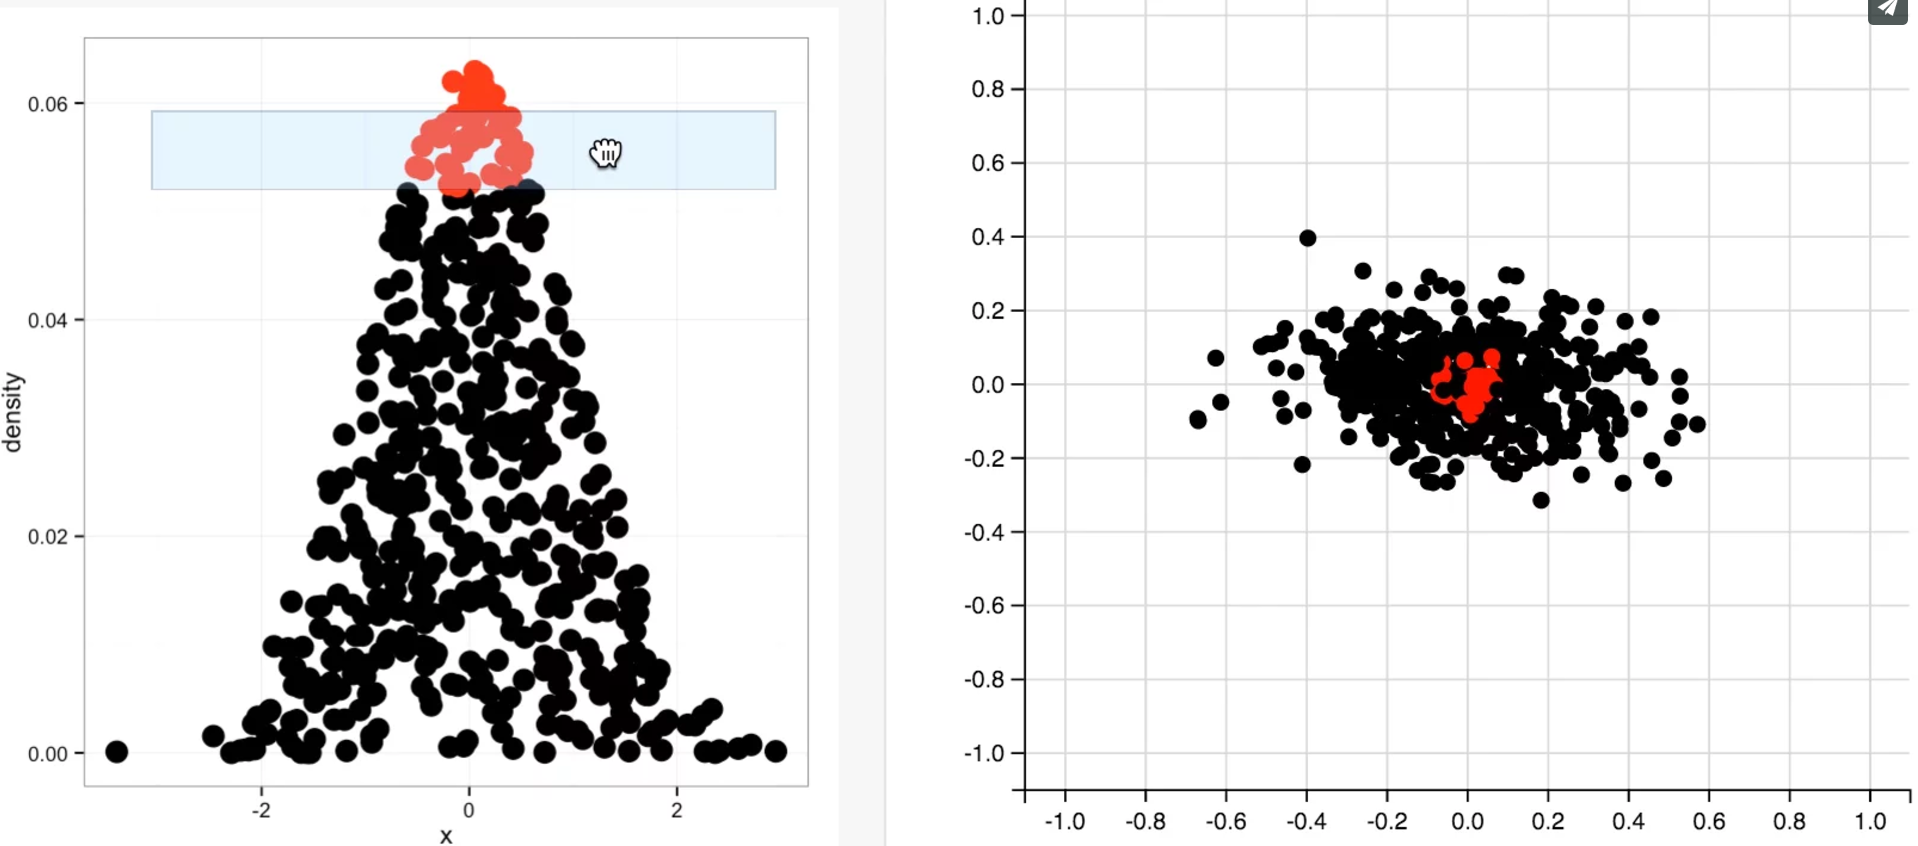
\includegraphics[width=26.64in]{diagrams/tourbrush} 

}

\caption{A demonstration of interactive and dynamic techniques for visualizing high-dimensional relationships in data using the R package **tourbrush**. You can view this movie online at <https://vimeo.com/148050343> or via the supplementary materials}\label{fig:tour}
\end{figure}

Dynamic interactive statistical graphics is useful for descriptive
statistics, and also to help build better inferential models. Any
statistician is familiar with diagnosing a model by plotting data in the
model space (e.g., residual plot, qqplot). This works well for
determining if the assumptions of a model are adequate, but rarely
suggests that our model neglects important features in the data. To
combat this problem, Wickham, Cook, and Hofmann (2015) suggest to plot
the model in the data space and use dynamic interactive statistical
graphics to do so. Interactive graphics have also proved to be useful
for exploratory model analysis, a situation where we have many models to
evaluate, compare, and critique (Unwin, Volinsky, and Winkler 2003);
(Urbanek 2004); (Ripley 2004); (Unwin 2006); (Wickham 2007). With such
power comes responsibility that we can verify that visual discoveries
are real, and not due to random chance (Buja et al. 2009); (Majumder,
Hofmann, and Cook 2013).

The ASA Section on Statistical Computing and Graphics maintains a video
library which captures many useful dynamic interactive statistical
graphics techniques. Several videos show how XGobi (predecessor to
GGobi), a dynamic interactive statistical graphics system, can be used
to reveal high-dimensional relationships and structures that cannot be
easily identified using numerical methods alone (Swayne, Cook, and Buja
1998).\footnote{For example,
  \url{http://stat-graphics.org/movies/xgobi.html} and
  \url{http://stat-graphics.org/movies/grand-tour.html}} Another notable
video shows how the interactive graphics system mondrian can be used to
quickly find interesting patterns in high-dimensional data using
exploratory data analysis (EDA) techniques (Theus and Urbanek
2008).\footnote{\url{http://stat-graphics.org/movies/tour-de-france.html}}
The most recent video shows how dynamic interactive techniques can help
interpret a topic model (a statistical mixture model applied to text
data) using the R package \textbf{LDAvis} (Sievert and Shirley 2014),
which is the first web-based visualization in the library, and is
discussed at depth in
\protect\hyperlink{ldavis-a-method-for-visualizing-and-interpreting-topics}{LDAvis:
A method for visualizing and interpreting topics}.

In order to be practically useful, interactive statistical graphics must
be fast, flexible, accessible, portable, and reproducible. In general,
over the last 20-30 years interactive graphics systems were fast and
flexible, but were generally not easily accessible, portable, or
reproducible. The web browser provides a convenient platform to combat
these problems. For example, any visualization created with
\textbf{LDAvis} can be shared through a Uniform Resource Locator (URL),
meaning that anyone with a web browser and an internet connection can
view and interact with a visualization. Furthermore, we can link anyone
to any possible state of the visualization by encoding selections with a
URL fragment identifier. This makes it possible to link readers to an
interesting state of a visualization from an external document, while
still allowing them to independently explore the same visualization and
assess conclusions drawn from it.\footnote{A good example of is
  \url{http://cpsievert.github.io/LDAvis/reviews/reviews.html}}

\subsection{Indirect versus direct
manipulation}\label{indirect-versus-direct-manipulation}

Even within the statistical graphics community, the term
\emph{interactive} graphics can mean wildly different things to
different people (Swayne and Klinke 1999). Some early statistical
literature on the topic uses interactive in the sense that an
interactive command-line prompt allows users to create graphics
on-the-fly (R. A. Becker 1984). That is, users enter commands into the
command-line prompt, the prompts evaluates the command, and prints the
result (known as the read--eval--print loop (REPL)). Modifying a command
to generate another variation of a particular result (e.g., to restyle a
static plot) can be thought of as a type of interaction that some might
call \emph{indirect manipulation}.

Indirect manipulation can be achieved both from the command-line or from
a graphical user interface (GUI). Indirect manipulation from the
command-line is more flexible since we have complete control over the
commands, but it is also more cumbersome since we must translate our
thoughts into code. Indirect manipulation via a GUI is more restrictive,
but it helps reduces the gulf of execution (i.e., easier to generate
desired output) for end-users (Hutchins, Hollan, and Norman 1985). In
this sense, a GUI can be useful, even for experienced programmers, when
the command-line interface impedes our primary task of deriving insight
from data.

In many cases, the gulf of execution can be further reduced through
direct manipulation. Roughly speaking, within the context of interactive
graphics, direct manipulation occurs whenever we interact with a plot
and reveal new information tied to the event. Cook and Swayne (2007) use
the terms dynamic graphics and direct manipulation to characterize
``plots that respond in real time to an analyst's queries and change
dynamically to re-focus, link to information from other sources, and
re-organize information.'' Directly manipulating multiple linked views
to make graphical queries is a very powerful framework for exploring
information, and inspires the last 3 chapters of this thesis.

A simple example to help demonstrate the differences between these
interactive techniques would be in an analysis of variance (ANOVA) via
multiple boxplots. By default, most plotting libraries sort categories
alphabetically, but this is usually not optimal for visual comparison of
groups. With a static plotting library such as \textbf{ggplot2}, we
could indirectly manipulate the default by going back to the
command-line, reordering the factor levels of the categorical variables,
and regenerate the plot (Wickham 2009). This is flexible and precise
since we may order the levels by any measure we wish (e.g., Median,
Mean, IQR, etc.), but it would be much quicker and easier if we had a
GUI with a drop-down menu for most of the reasonable sorting options. In
a general purpose interactive graphics system such as mondrian, one can
use direct manipulation to directly click and drag on the categories to
reorder them, making it quick and easy to compare any two groups of
interest (Theus and Urbanek 2008).

\subsection{Multiple linked views}\label{multiple-linked-views}

A general purpose interactive statistical graphics system should possess
many direct manipulation techniques such as identifying (i.e., mousing
over points to reveal labels), focusing (i.e., view size adjustment, pan
and zoom), brushing/identifying, etc. However, it is the intricate
management of information across multiple views of data in response to
user events that is most valuable. Extending ideas from (Andreas Buja
and McDonald 1988), (Wickham et al. 2010) point out that any
visualization system with linked views must implement a data pipeline.
That is, a ``central commander'' must be able to handle interaction(s)
with a given view, translate its meaning to the data space, and update
any linked view(s) accordingly. In order to do so, the commander must
know, and be able to compute, function(s) from data to visual space, as
well as from visual space to the data. Implementing a pipeline that is
fast, general, and able to handle statistical transformations is
incredibly difficult. Unfortunately, literature on the implementation of
such pipelines is virtually non-existent, but Xie, Hofmann, and Cheng
(2014) provides a nice overview of the implementation details in the R
package \textbf{cranvas} (Yihui Xie 2013).

\subsection{Web graphics}\label{web-graphics}

Thanks to the constant evolution and eventual adoption of HTML5 as a web
standard, the modern web browser now provides a viable platform for
building an interactive statistical graphics systems. HTML5 refers to a
collection of technologies, each designed to perform a certain task,
that work together in order to present content in a web browser. The
Document Object Model (DOM) is a convention for managing all of these
technologies to enable \emph{dynamic} and \emph{interactive} web pages.
Among these technologies, there are several that are especially relevant
for interactive web graphics:

\begin{enumerate}
\def\labelenumi{\arabic{enumi}.}
\tightlist
\item
  HTML: A markup language for structuring and presenting web content.
\item
  SVG: A markup language for drawing scalable vector graphics.
\item
  CSS: A language for specifying styling of web content.
\item
  JavaScript: A language for manipulating web content.
\end{enumerate}

Juggling all of these technologies just to create a simple statistical
plot is a tall order. Thankfully, HTML5 technologies are publicly
available, and benefit from thriving community of open source developers
and volunteers. In the context of web-based visualization, the most
influential contribution is Data Driven Documents (D3), a JavaScript
library which provides high-level semantics for binding data to web
content (e.g., SVG elements) and orchestrating scene updates/transitions
(Heer 2011). D3 is wildly successful because is builds upon web
standards, without abstracting them away, which fosters customization
and interoperability. However, compared to a statistical graphics
environments like R, creating basic charts is complicated, and a large
amount of code must be hard-wired to each visualization. Fortunately,
there are a number of ways to provide higher-level interfaces to web
graphics, and we focus on R interfaces.

\subsection{Translating R graphics to the
web}\label{translating-r-graphics-to-the-web}

There are a few ways to simply translate R graphics to a web format,
such as SVG. R has built-in support for a SVG graphics device, made
available through the \texttt{svg()} function, but it can be quite slow,
which inspired the new \textbf{svglite} package (Wickham et al. 2016).
The \textbf{SVGAnnotation} package provides some functionality to
post-process SVG files generated with \texttt{svg()} to add some basic
interactivity and animation (Nolan and Temple Lang 2012). The
\textbf{gridSVG} package is specially designed to translate
\textbf{grid} graphics (e.g., \textbf{ggplot2}, \textbf{lattice}, etc.)
to SVG, and preserves the naming information of grid objects, making it
easier to layer on interactive functionality (Potter and Murrell 2012).
Fujino (2015) uses \textbf{gridSVG} to enable linked brushing between
\textbf{ggplot2} graphics, but only implements a few chart types. Riutta
et. al. and Russell (2015) uses \textbf{gridSVG} to provide pan and zoom
capability to virtually any R graphic.

The \textbf{animint} and \textbf{plotly} packages take a different
approach to translating \textbf{ggplot2} graphics to a web format
(Hocking, VanderPlas, and Sievert 2015); (Sievert et al. 2016). Instead
of translating directly to SVG via \textbf{gridSVG}, they extract
relevant information from the internal representation of a
\textbf{ggplot2} graphic\footnote{For a visual display of the internal
  representation used to render a \textbf{ggplot2} graph, see my
  \textbf{shiny} app here \url{https://gallery.shinyapps.io/ggtree}.},
store it in JavaScript Object Notation (JSON), and pass the JSON as
input to a JavaScript function, which then produces a web based
visualization. It is becoming more and more popular to see JavaScript
graphing libraries use this design pattern (sometimes referred to as a
JSON specification or schema), since it separates out \emph{what}
information is contained in the graphic from \emph{how} to actually draw
it. This has a number of advantages; for example, \textbf{plotly}
graphics can be rendered in SVG, or using WebGL (based on HTML5 canvas,
not SVG) which allows the browser to render many more graphical marks by
leveraging the GPU.

Converting static graphics to web formats such as SVG or canvas not only
allows us to embed the graphics into larger HTML documents, but it also
allows us to inject basic interactive features at no or little cost to
the user. For example, in both \textbf{animint} and \textbf{plotly}, we
provide tool-tips (to obtain data-related information for each graphical
mark) and clickable legends that show/hide graphical marks corresponding
to the legend entry. In the case of \textbf{animint}, we have also
extended \textbf{ggplot2}'s grammar of graphics implementation to enable
animations and categorical linking between plots with relatively small
amount of effort by users. This extension is discussed at length in
\protect\hyperlink{two-new-keywords-for-interactive-animated-plot-design-clickSelects-and-showSelected}{Two
new keywords for interactive, animated plot design: clickSelects and
showSelected}. In the case of \textbf{plotly}, we have also enabled
animations, highlighting, and linked highlighting (even between
non-plotly graphics). These features are discussed at length in
\href{https://cpsievert.github.io/plotly_book/}{plotly for R}.

\subsection{R interfaces for interactive web
graphics}\label{r-interfaces-for-interactive-web-graphics}

Translating existing graphics to a web-based format is useful for
quickly breathing new life into existing code, but it is fairly limited
in how far we can take it. Assuming the goal is to have a general, yet
high-level, interface for creating highly dynamic interactive web
graphics from R, we're better off building a new interface designed
exactly for this purpose. The first serious attempt in this direction
was the R package \textbf{rCharts}, whose R interface is heavily
inspired by \textbf{lattice} (Vaidyanathan 2013). The most impressive
result of \textbf{rCharts}'s design is its ability to interface with
many different JavaScript charting libraries. However, \textbf{rCharts}
has little to no support for coordination of dynamic linked views from
R.

Another notable interface for creating interactive web graphics from R
is \textbf{ggvis}, a reworking of ggplot2's grammar of graphics to
incorporate interactivity (Chang and Wickham 2015). Similar to
\textbf{animint}, \textbf{ggvis} encodes plot specific information as
JSON, but instead of writing a JavaScript renderer from the ground up,
it uses Vega, a popular JSON schema for creating web-based graphics
(Heer 2014). This limits the flexibility of \textbf{ggvis}, but it also
drastically reduces the overhead in maintaining such a software project,
allowing the focus to be on building a grammar for expressing
interactions from R.

The current version of \textbf{ggvis} uses an old version of vega,
before a grammar for interactive graphics was added to its JSON schema
(Heer 2017). In order to respond to user interactions with vega
graphics, \textbf{ggvis} has its own custom JavaScript designed
specifically for vega. To enable support for coordinated linked views,
it exposes the data pipeline to users via the R package \textbf{shiny},
a framework for writing web applications in R (Chang et al. 2015). A web
application is a website which, when visited by users (aka clients),
communicates with a web server. This approach is useful when a website
needs to execute code that can not be executed in the web browser (e.g.,
R code). Figure \ref{fig:server-client} provides a visual demonstration
of this model and its relation to the data pipeline necessary for
coordinating linked views.

\begin{figure}

{\centering 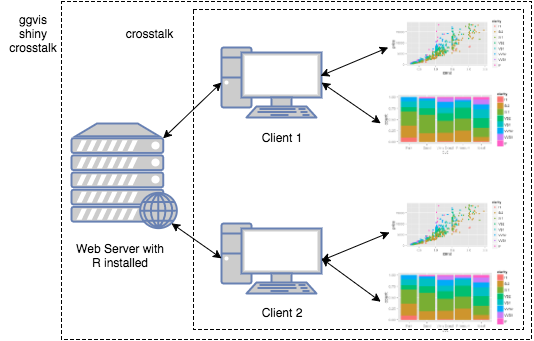
\includegraphics{diagrams/server-client} 

}

\caption{A basic visual depiction of the different approaches to implementing a data pipeline for interactive web graphics. The R packages **ggvis** and **shiny** expose the pipeline to users in R, which requires a web server for viewing. The R package **crosstalk** will allow developers to implement and expose the pipeline on both the server and client levels.}\label{fig:server-client}
\end{figure}

Generally speaking, websites that render entirely client-side are more
desirable since they are easier to share, more responsive, and require
less computational resources to run\footnote{The
  \url{http://www.shinyapps.io/} service helps to provide easy access to
  a \textbf{shiny} server (a web server running special shiny software),
  so that \textbf{shiny} apps can be shared via a URL, for example:
  \url{https://hadley.shinyapps.io/14-ggvis/linked-brushing.Rmd}}.
However, the client-server approach can be very useful for dynamically
performing statistical computations, a key characteristic of most
interactive statistical graphics systems. (Urbanek and Horner 2015) and
(Jeroen Ooms 2014b) also allow us to execute R code on a web server, and
retrieve output via HTTP, but \textbf{shiny} is the most heavily used
since apps can be written entirely in R using a very powerful, yet
approachable, reactive programming framework for handling user events.
There are also many convenient shortcuts for creating attractive HTML
input forms, making it incredibly easy to go from R script to an web app
powered by R that dynamically updates when users alter input values. In
other words, \textbf{shiny} makes it quick and easy to write web-based
GUIs with support for indirect manipulation.

Historically, an advanced understanding of \textbf{shiny} and JavaScript
was required to implement direct manipulation in a \textbf{shiny} app.
Recently, \textbf{shiny} added support for retrieving information on
user events with static R graphics\footnote{This website shows what
  information is sent from the client to the server when users interact
  with plot(s) via mouse event(s) --
  \url{http://shiny.rstudio.com/gallery/plot-interaction-basic.html}},
allowing developers to coordinate views in a web app, with no JavaScript
involved. This is a powerful tool for R users, but it has its
weaknesses. Most importantly, its not clear how to handle interactions
when positional scales are categorical (e.g., a bar chart) or how to
provide a visual clue that something has been selected.

The touring video in Figure \ref{fig:tour} purposefully uses
\textbf{shiny}'s built-in support for brushing to demonstrate the
problem with providing a visual clue. This points to the fundamental
problem in using non-web-based graphics to implement interactive
graphics in a web browser: every time the view updates, the display must
be redrawn, resulting in a ``glitch'' effect. If the plot being brushed
used native web graphics (e.g., SVG), it would allow for finer control
over how the view updates in response to user interactions and/or
dynamic data. On the other hand, since \textbf{ggvis} is web-based, and
has special client-side functionality, it knows how to smoothly
transition from one frame to the next when provided with new data from
the \textbf{shiny} server, which is crucial for constructing a mental
model of the data space. Having richer interfaces for generating
web-based interactive graphics from R that can share selections, and
handle smooth transitions, would make this, and many other examples,
generally better.

Many web-based graphing toolkits have appeared since the advent of
\textbf{rCharts}, making a single package that interfaces with
\emph{every} toolkit infeasible. Some ideas deriving from work on
\textbf{rCharts}, such as providing the glue to render plots in various
contexts (e.g., the R console, shiny apps, and \textbf{rmarkdown}
documents), have evolved into the R package \textbf{htmlwidgets}
(Vaidyanathan et al. 2015). Having built similar bridges for
\textbf{animint} and \textbf{LDAvis}, I personally know and appreciate
the amount of time and effort this package saves other package authors.

The \textbf{htmlwidgets} framework is not constrained to just graphics,
it simply provides a set of conventions for authoring web content from
R. Numerous JavaScript data visualization libraries are now made
available using this framework, most designed for particular use cases,
such as \textbf{leaflet} for geo-spatial mapping, \textbf{dygraphs} for
time-series, and \textbf{networkD3} for networks (Cheng and Xie 2015);
(Vanderkam and Allaire 2015); (Gandrud, Allaire, and Russell
2015).\footnote{For more examples and information, see
  \url{http://www.htmlwidgets.org/} and
  \url{http://hafen.github.io/htmlwidgetsgallery/}} There are also HTML
widgets that provide an interface to more general purpose visualization
JavaScript libraries such as \textbf{plotly}, \textbf{rbokeh}, and
\textbf{rcdimple} (Sievert et al. 2016); (Hafen and team 2015);
(Kiernander et al. 2015). Most of these JavaScript libraries provide at
least some native support for direct manipulation such as identifying
(i.e., mousing over points to reveal labels), focusing (i.e., pan and
zoom), and sometimes highlighting (i.e., brushing over points to
highlight points in another view). More often than not, the support for
dynamic and linked views is lacking, especially if we want to define the
linking in R, and produce a standalone HTML document.

The R package \textbf{crosstalk} is a new framework for coordinating
arbitrary HTML widgets (Cheng 2015a). It provides both an R and a
JavaScript API for querying selections, meaning \textbf{crosstalk}
powered HTML widgets can work with or without \textbf{shiny}, and if
implemented carefully by HTML widget authors, provides a means for
coordinating multiple HTML widgets without shiny. Generally speaking,
\textbf{crosstalk} just provides a standard way to set, store, and
access selection values in the browser, so the actual logic for updating
views based on the selection value(s) is on the HTML widget author, and
this part is far from trivial. In a sense, this project is similar to
the work of North and Shneiderman (1999), which provides semantics for
``snapping together'' arbitrary views that are aware of the relational
schema, but does so in a web-based environment, rather than requiring a
machine running Windows.

The first HTML widget to leverage \textbf{crosstalk} was (Cheng 2015b),
but is limited to linked brushing on scatterplots.\footnote{See, for
  example, \url{http://rpubs.com/jcheng/crosstalk-demo}} Currently,
there are a couple other R packages with \textbf{crosstalk} support,
including \textbf{leaflet} and \textbf{listviewer}, but \textbf{plotly}
is the only package which supports a non-identity functions between the
data and displays. It also has rich support for interaction types,
including mouse hover, click, and multiple types of click+drag
selections.

Having HTML widgets that can share selections with each other will be a
huge step forward for web-based interactive graphics. With some effort
and careful implementation by HTML widget authors, it may be possible to
provide sensible defaults for updating views between arbitrary widgets,
and users that know some JavaScript will also be able to customize or
extend these defaults from R. The \textbf{htmlwidget} package provides
conventions for this, by allowing one to send arbitrary JavaScript
functions from R that execute after the widget has rendered in the
browser. The biggest problem in implementing coordinated widgets will be
in managing data structures, since each widget will likely have its own
data structure for representing a selection. In this case, in order to
coordinate them, users may have to embed widgets in a shiny app to
access and organize selections. This gives users tremendous control over
sharing selections, but may limit control over smooth transitions
between states of a given widget (a key characteristic of dynamic
graphics), and increases the amount of complexity involved in sharing
their work.

\chapter{Taming PITCHf/x Data with XML2R and pitchRx}

\textbf{XML2R} is a framework that reduces the effort required to
transform XML content into tables in a way that preserves parent to
child relationships. \textbf{pitchRx} applies \textbf{XML2R}'s grammar
for XML manipulation to Major League Baseball Advanced Media (MLBAM)'s
Gameday data. With \textbf{pitchRx}, one can easily obtain and store
Gameday data in a remote database. The Gameday website hosts a wealth of
XML data, but perhaps most interesting is PITCHf/x. Among other things,
PITCHf/x data can be used to recreate a baseball's flight path from a
pitcher's hand to home plate. With \textbf{pitchRx}, one can easily
create animations and interactive 3D scatterplots of the baseball's
flight path. PITCHf/x data is also commonly used to generate a static
plot of baseball locations at the moment they cross home plate. These
plots, sometimes called \textit{strike-zone plots}, can also refer to a
plot of event probabilities over the same region. \textbf{pitchRx}
provides an easy and robust way to generate strike-zone plots using the
\textbf{ggplot2} package.

\section{Introduction}\label{introduction}

\subsection{What is PITCHf/x?}\label{what-is-pitchfx}

PITCHf/x is a general term for a system that generates a series of 3D
measurements of a baseball's path from a pitcher's hand to home plate
(Alt and White 2008).
\footnote{A \textit{pitcher} throws a ball to the opposing \textit{batter}, who
stands besides home plate and tries to hit the ball into the field
of play.
} In an attempt to estimate the location of the ball at any time point,
a quadratic regression model with nine parameters (defined by the
equations of motion for constant linear acceleration) is fit to each
pitch. Studies with access to the actual measurements suggest that this
model is quite reasonable -- especially for non-knuckleball pitches
(Nathan 2008). That is, the fitted path often provides a reasonable
estimate (within a couple of inches) of the actual locations.
Unfortunately, only the parameter estimates are made available to the
public. The website that provides these estimates is maintained by MLBAM
and hosts a wealth of other baseball related data used to inform MLB's
Gameday webcast service in near real time.

\subsection{Why is PITCHf/x important?}\label{why-is-pitchfx-important}

On the business side of baseball, using statistical analysis to scout
and evaluate players has become mainstream. When PITCHf/x was first
introduced, DiMeo (2007) proclaimed it as,

\begin{quote} ``The new technology that will change statistical analysis [of baseball] forever.'' \end{quote}

PITCHf/x has yet to fully deliver this claim, partially due to the
difficulty in accessing and deriving insight from the large amount of
complex information. By providing better tools to collect and visualize
this data, \textbf{pitchRx} makes PITCHf/x analysis more accessible to
the general public.

\subsection{PITCHf/x applications}\label{pitchfx-applications}

PITCHf/x data is and can be used for many different projects. It can
also complement other baseball data sources, which poses an interesting
database management problem. Statistical analysis of PITCHf/x data and
baseball in general has become so popular that it has helped expose
statistical ideas and practice to the general public. If you have
witnessed television broadcasts of MLB games, you know one obvious
application of PITCHf/x is locating pitches in the strike-zone as well
as recreating flight trajectories, tracking pitch speed, etc. Some
on-going statistical research related to PITCHf/x includes: classifying
pitch types, predicting pitch sequences, and clustering pitchers with
similar tendencies (Pane et al. 2013).

\subsection[Contributions of pitchRx and XML2R]{Contributions of \textbf{pitchRx} and \textbf{XML2R}}

The \textbf{pitchRx} package has two main focuses (Sievert 2014a). The
first focus is to provide easy access to Gameday data. Not only is
\textbf{pitchRx} helpful for collecting this data in bulk, but it has
served as a helpful teaching and research aide
(\url{http://baseballwithr.wordpress.com/} is one such example). Methods
for collecting Gameday data existed prior to \textbf{pitchRx}; however,
these methods are not easily extensible and require juggling
technologies that may not be familiar or accessible (Fast 2007).
Moreover, these working environments are less desirable than R for data
analysis and visualization. Since \textbf{pitchRx} is built upon
\textbf{XML2R}'s united framework, it can be easily modified and/or
extended (Sievert 2014c). For this same reason, \textbf{pitchRx} serves
as a model for building customized XML data collection tools with
\textbf{XML2R}.

The other main focus of \textbf{pitchRx} is to simplify the process
creating popular PITCHf/x graphics. Strike-zone plots and animations
made via \textbf{pitchRx} utilize the extensible \textbf{ggplot2}
framework as well as various customized options (Wickham 2009).
\textbf{ggplot2} is a convenient framework for generating strike-zone
plots primarily because of its facet schema which allows one to make
visual comparisons across any combination of discrete variable(s).
Interactive 3D scatterplots are based on the \textbf{rgl} package and
useful for gaining a new perspective on flight trajectories (Adler,
Murdoch, and others, n.d.).

\section{Getting familiar with
Gameday}\label{getting-familiar-with-gameday}

Gameday data is hosted and made available for free thanks to MLBAM via
\url{http://gd2.mlb.com/components/game/mlb/}.
\footnote{Please be respectful of this service and store any information after
you extract it instead of repeatedly querying the website. Before
using any content from this website, please also read the \href{http://gdx.mlb.com/components/copyright.txt}{copyright}.
} From this website, one can obtain many different types of data besides
PITCHf/x. For example, one can obtain everything from
\href{http://gd2.mlb.com/components/game/mlb/year_2013/month_07/day_16/gid_2013_07_16_aasmlb_nasmlb_1/media/instadium.xml}{structured media metadata}
to
\href{http://gd2.mlb.com/components/game/mlb/twitter/anaInsiderTweets.xml}{insider tweets}.
In fact, this website's purpose is to serve data to various
\url{http://mlb.com} web pages and applications. As a result, some data
is redundant and the format may not be optimal for statistical analysis.
For these reasons, the \texttt{scrape} function is focused on retrieving
data that is useful for PITCHf/x analysis and providing it in a
convenient format for data analysis.

Navigating through the MLBAM website can be overwhelming, but it helps
to recognize that a homepage exists for nearly every day and every game.
For example,
\url{http://gd2.mlb.com/components/game/mlb/year_2011/month_02/day_26/}
displays numerous hyperlinks to various files specific to February 26th,
2011. On this page is a hyperlink to
\href{http://gd2.mlb.com/components/game/mlb/year_2011/month_02/day_26/miniscoreboard.xml}{miniscoreboard.xml}
which contains information on every game played on that date. This page
also has numerous hyperlinks to game specific pages. For example,
\href{http://gd2.mlb.com/components/game/mlb/year_2011/month_02/day_26/gid_2011_02_26_phimlb_nyamlb_1/}{gid\_2011\_02\_26\_phimlb\_nyamlb\_1/}
points to the homepage for that day's game between the NY Yankees and
Philadelphia Phillies. On this page is a hyperlink to the
\href{http://gd2.mlb.com/components/game/mlb/year_2011/month_02/day_26/gid_2011_02_26_phimlb_nyamlb_1/players.xml}{players.xml}
file which contains information about the players, umpires, and coaches
(positions, names, batting average, etc.) coming into that game.

Starting from a particular game's homepage and clicking on the
\href{http://gd2.mlb.com/components/game/mlb/year_2011/month_02/day_26/gid_2011_02_26_phimlb_nyamlb_1/inning/}{inning/}
directory, we \emph{should} see another page with links to the
\href{http://gd2.mlb.com/components/game/mlb/year_2011/month_02/day_26/gid_2011_02_26_phimlb_nyamlb_1/inning/inning_all.xml}{inning\_all.xml}
file and the
\href{http://gd2.mlb.com/components/game/mlb/year_2011/month_02/day_26/gid_2011_02_26_phimlb_nyamlb_1/inning/inning_hit.xml}{inning\_hit.xml}
file. If it is available, the \texttt{inning\_all.xml} file contains the
PITCHf/x data for that game. It's important to note that this file won't
exist for some games, because some games are played in venues that do
not have a working PITCHf/x system in place. This is especially true for
preseason games and games played prior to the 2008 season when the
PITCHf/x system became widely adopted.
\footnote{In this case, \texttt{scrape} will print ``failed to load HTTP resource''
in the R console (after the relevant file name) to indicate that no
data was available.
} The \texttt{inning\_hit.xml} files have manually recorded spatial
coordinates of where a home run landed or where the baseball made
initial contact with a defender after it was hit into play.

The relationship between these XML files and the tables returned by
\texttt{scrape} is presented in
Table\textasciitilde{}\ref{table:pitchfx}. The \texttt{pitch} table is
extracted from files whose name ends in \texttt{inning\_all.xml}. This
is the only table returned by \texttt{scrape} that contains data on the
pitch-by-pitch level. The \texttt{atbat}, \texttt{runner},
\texttt{action} and \texttt{hip} tables from this same file are commonly
labeled somewhat ambiguously as play-by-play data. The \texttt{player},
\texttt{coach}, and \texttt{umpire} tables are extracted from
\texttt{players.xml} and are classified as game-by-game since there is
one record per person per game. Figure \ref{fig:relations} shows how
these tables can be connected to one another in a database setting. The
direction of the arrows represent a one to possibly many relationship.
For example, at least one pitch is thrown for each \textit{at bat} (that
is, each bout between pitcher and batter) and there are numerous at bats
within each game.

In a rough sense, one can relate tables returned by \texttt{scrape} back
to XML nodes in the XML files. For convenience, some information in
certain XML nodes are combined into one table. For example, information
gleaned from the `top', `bottom', and `inning' XML nodes within
\texttt{inning\_all.xml} are included as \texttt{inning} and
\texttt{inning\_side} fields in the \texttt{pitch}, \texttt{po},
\texttt{atbat}, \texttt{runner}, and \texttt{action} tables. This helps
reduce the burden of merging many tables together in order to have
inning information on the play-by-play and/or pitch-by-pitch level.
Other information is simply ignored simply because it is redundant. For
example, the `game' node within the \texttt{players.xml} file contains
information that can be recovered from the \texttt{game} table extracted
from the \texttt{miniscoreboard.xml} file. If the reader wants a more
detailed explanation of fields in these tables, Marchi and Albert (2013)
provide nice overview.

\section{Introducing XML2R}\label{introducing-xml2r}

\textbf{XML2R} adds to the
\href{http://cran.r-project.org/web/views/WebTechnologies.html}{CRAN Task View on Web Technologies and Services}
by focusing on the transformation of XML content into a collection of
tables. Compared to a lower-level API like the \textbf{XML} package, it
can significantly reduce the amount of coding and cognitive effort
required to perform such a task. In contrast to most higher-level APIs,
it does not make assumptions about the XML structure or its source.
Although \textbf{XML2R} works on any structure, performance and user
experience are enhanced if the content has an inherent relational
structure. \textbf{XML2R}'s novel approach to XML data collection breaks
down the transformation process into a few simple steps and allows the
user to decide how to apply those steps.

The next few sections demonstrate how \textbf{pitchRx} leverages
\textbf{XML2R} in order to produce a collection of tables from
\texttt{inning\_all.xml} files. A similar approach is used by
\texttt{pitchRx::scrape} to construct tables from the other Gameday
files in Table\textasciitilde{}\ref{table:pitchfx}. In fact,
\textbf{XML2R} has also been used in the R package
\href{https://github.com/cpsievert/bbscrapeR}{bbscrapeR} which collects
data from \href{http://nba.com}{nba.com} and
\href{http://wnba.com}{wnba.com}.

\subsection{Constructing file names}\label{constructing-file-names}

Sometimes the most frustrating part of obtaining data in bulk off of the
web is finding the proper collection of URLs or file names of interest.
Since files on the Gameday website are fairly well organized, the
\texttt{makeUrls} function can be used to construct \texttt{urls} that
point to every game's homepage within a window of dates.

\begin{Shaded}
\begin{Highlighting}[]
\NormalTok{urls <-}\StringTok{ }\KeywordTok{makeUrls}\NormalTok{(}\DataTypeTok{start =} \StringTok{"2011-06-01"}\NormalTok{, }\DataTypeTok{end =} \StringTok{"2011-06-01"}\NormalTok{) }
\KeywordTok{sub}\NormalTok{(}\StringTok{"http://gd2.mlb.com/components/game/mlb/"}\NormalTok{, }\StringTok{""}\NormalTok{, }\KeywordTok{head}\NormalTok{(urls))}
\end{Highlighting}
\end{Shaded}

\begin{Shaded}
\begin{Highlighting}[]
\CommentTok{#> [1] "year_2011/month_06/day_01/gid_2011_06_01_anamlb_kcamlb_1"}
\CommentTok{#> [2] "year_2011/month_06/day_01/gid_2011_06_01_balmlb_seamlb_1"}
\CommentTok{#> [3] "year_2011/month_06/day_01/gid_2011_06_01_chamlb_bosmlb_1"}
\CommentTok{#> [4] "year_2011/month_06/day_01/gid_2011_06_01_clemlb_tormlb_1"}
\CommentTok{#> [5] "year_2011/month_06/day_01/gid_2011_06_01_colmlb_lanmlb_1"}
\CommentTok{#> [6] "year_2011/month_06/day_01/gid_2011_06_01_flomlb_arimlb_1"}
\end{Highlighting}
\end{Shaded}

\subsection{Extracting observations}\label{extracting-observations}

Once we have a collection of XML \texttt{files}, the next step is to
parse the content into a list of \textit{observations}. An observation
is technically defined as a matrix with one row and some number of
columns. The columns are defined by XML attributes and the XML value (if
any) for a particular XML lineage. The name of each observation tracks
the XML hierarchy so observations can be grouped together in a sensible
fashion at a later point.

\begin{Shaded}
\begin{Highlighting}[]
\KeywordTok{library}\NormalTok{(XML2R)}
\NormalTok{files <-}\StringTok{ }\KeywordTok{paste0}\NormalTok{(urls, }\StringTok{"/inning/inning_all.xml"}\NormalTok{)}
\NormalTok{obs <-}\StringTok{ }\KeywordTok{XML2Obs}\NormalTok{(files, }\DataTypeTok{url.map =} \OtherTok{TRUE}\NormalTok{, }\DataTypeTok{quiet =} \OtherTok{TRUE}\NormalTok{) }
\KeywordTok{table}\NormalTok{(}\KeywordTok{names}\NormalTok{(obs))}
\end{Highlighting}
\end{Shaded}

\begin{Shaded}
\begin{Highlighting}[]
\CommentTok{#> }
\CommentTok{#>                                game                        game//inning }
\CommentTok{#>                                   2                                  18 }
\CommentTok{#>        game//inning//bottom//action         game//inning//bottom//atbat }
\CommentTok{#>                                  13                                  69 }
\CommentTok{#>  game//inning//bottom//atbat//pitch     game//inning//bottom//atbat//po }
\CommentTok{#>                                 247                                   4 }
\CommentTok{#> game//inning//bottom//atbat//runner           game//inning//top//action }
\CommentTok{#>                                  50                                  20 }
\CommentTok{#>            game//inning//top//atbat     game//inning//top//atbat//pitch }
\CommentTok{#>                                  79                                 278 }
\CommentTok{#>        game//inning//top//atbat//po    game//inning//top//atbat//runner }
\CommentTok{#>                                  17                                  89 }
\CommentTok{#>                             url_map }
\CommentTok{#>                                   1}
\end{Highlighting}
\end{Shaded}

This output tells us that 247 pitches were thrown in the bottom inning
and 278 were thrown in the top inning on June 1st, 2011. Also, there are
12 different levels of observations. The list element named
\texttt{url\_map} is not considered an observation and was included
since \texttt{url.map = TRUE}. This helps avoid repeating long file
names in the \texttt{url\_key} column which tracks the mapping between
observations and file names.

\begin{Shaded}
\begin{Highlighting}[]
\NormalTok{obs[}\DecValTok{1}\NormalTok{]}
\end{Highlighting}
\end{Shaded}

\begin{Shaded}
\begin{Highlighting}[]
\CommentTok{#> $`game//inning//top//atbat//pitch`}
\CommentTok{#>      des             id  type tfs      tfs_zulu               x        y       }
\CommentTok{#> [1,] "Called Strike" "3" "S"  "191018" "2011-06-01T23:10:18Z" "109.87" "145.06"}
\CommentTok{#>      sv_id           start_speed end_speed sz_top sz_bot pfx_x  pfx_z  px      }
\CommentTok{#> [1,] "110601_191020" "87.9"      "82.1"    "3.6"  "1.65" "-6.7" "4.36" "-0.213"}
\CommentTok{#>      pz      x0       y0     z0      vx0     vy0        vz0      ax       }
\CommentTok{#> [1,] "2.611" "-1.612" "50.0" "5.633" "5.808" "-128.728" "-2.903" "-11.406"}
\CommentTok{#>      ay       az        break_y break_angle break_length pitch_type}
\CommentTok{#> [1,] "22.954" "-24.681" "23.9"  "22.5"      "6.5"        "SI"      }
\CommentTok{#>      type_confidence zone nasty spin_dir  spin_rate  cc mt url_key}
\CommentTok{#> [1,] ".798"          "5"  "39"  "236.697" "1538.041" "" "" "url1"}
\end{Highlighting}
\end{Shaded}

\subsection{Renaming observations}\label{renaming-observations}

Before grouping observations into a collection tables based on their
names, one may want to \texttt{re\_name} observations. Observations with
names \texttt{'game//inning//bottom//atbat'} and
\texttt{'game//inning//top//atbat'} should be included in the same table
since they share XML attributes (in other words, the observations share
variables).

\begin{Shaded}
\begin{Highlighting}[]
\NormalTok{tmp <-}\StringTok{ }\KeywordTok{re_name}\NormalTok{(obs, }\DataTypeTok{equiv =} \KeywordTok{c}\NormalTok{(}\StringTok{"game//inning//top//atbat"}\NormalTok{,                             }
  \StringTok{"game//inning//bottom//atbat"}\NormalTok{), }\DataTypeTok{diff.name =} \StringTok{"inning_side"}\NormalTok{) }
\end{Highlighting}
\end{Shaded}

By passing these names to the \texttt{equiv} argument, \texttt{re\_name}
determines the difference in the naming scheme and suppresses that
difference. In other words, observation names that match the
\texttt{equiv} argument will be renamed to
\texttt{'game//inning//atbat'}. The information removed from the name is
not lost; however, as a new column is appended to the end of each
relevant observation. For example, notice how the \texttt{inning\_side}
column contains the part of the name we just removed:

\begin{Shaded}
\begin{Highlighting}[]
\NormalTok{tmp[}\KeywordTok{grep}\NormalTok{(}\StringTok{"game//inning//atbat"}\NormalTok{, }\KeywordTok{names}\NormalTok{(tmp))][}\DecValTok{1}\NormalTok{:}\DecValTok{2}\NormalTok{]}
\end{Highlighting}
\end{Shaded}

\begin{Shaded}
\begin{Highlighting}[]
\CommentTok{#> $`game//inning//atbat`}
\CommentTok{#>      num b   s   o   start_tfs start_tfs_zulu         batter   stand b_height}
\CommentTok{#> [1,] "1" "0" "1" "0" "190935"  "2011-06-01T23:09:35Z" "430001" "R"   "5-10"  }
\CommentTok{#>      pitcher  p_throws}
\CommentTok{#> [1,] "502190" "R"     }
\CommentTok{#>      des                                                       event      score}
\CommentTok{#> [1,] "Rickie Weeks homers (10) on a fly ball to left field.  " "Home Run" "T"  }
\CommentTok{#>      home_team_runs away_team_runs url_key inning_side}
\CommentTok{#> [1,] "0"            "1"            "url1"  "top"      }
\CommentTok{#> }
\CommentTok{#> $`game//inning//atbat`}
\CommentTok{#>      num b   s   o   start_tfs start_tfs_zulu         batter   stand b_height}
\CommentTok{#> [1,] "2" "0" "0" "0" "191105"  "2011-06-01T23:11:05Z" "460579" "L"   "6-0"   }
\CommentTok{#>      pitcher  p_throws}
\CommentTok{#> [1,] "502190" "R"     }
\CommentTok{#>      des                                                                     }
\CommentTok{#> [1,] "Nyjer Morgan triples (3) on a line drive to right fielder Jay Bruce.  "}
\CommentTok{#>      event    url_key inning_side}
\CommentTok{#> [1,] "Triple" "url1"  "top"}
\end{Highlighting}
\end{Shaded}

For similar reasons, other observation name pairs are renamed in a
similar fashion.

\begin{Shaded}
\begin{Highlighting}[]
\NormalTok{tmp <-}\StringTok{ }\KeywordTok{re_name}\NormalTok{(tmp, }\DataTypeTok{equiv =} \KeywordTok{c}\NormalTok{(}\StringTok{"game//inning//top//atbat//runner"}\NormalTok{,                             }
  \StringTok{"game//inning//bottom//atbat//runner"}\NormalTok{), }\DataTypeTok{diff.name =} \StringTok{"inning_side"}\NormalTok{)}
\NormalTok{tmp <-}\StringTok{ }\KeywordTok{re_name}\NormalTok{(tmp, }\DataTypeTok{equiv =} \KeywordTok{c}\NormalTok{(}\StringTok{"game//inning//top//action"}\NormalTok{,                             }
  \StringTok{"game//inning//bottom//action"}\NormalTok{), }\DataTypeTok{diff.name =} \StringTok{"inning_side"}\NormalTok{)  }
\NormalTok{tmp <-}\StringTok{ }\KeywordTok{re_name}\NormalTok{(tmp, }\DataTypeTok{equiv =} \KeywordTok{c}\NormalTok{(}\StringTok{"game//inning//top//atbat//po"}\NormalTok{,                            }
  \StringTok{"game//inning//bottom//atbat//po"}\NormalTok{), }\DataTypeTok{diff.name =} \StringTok{"inning_side"}\NormalTok{)}
\NormalTok{obs2 <-}\StringTok{ }\KeywordTok{re_name}\NormalTok{(tmp, }\DataTypeTok{equiv =} \KeywordTok{c}\NormalTok{(}\StringTok{"game//inning//top//atbat//pitch"}\NormalTok{,                             }
  \StringTok{"game//inning//bottom//atbat//pitch"}\NormalTok{), }\DataTypeTok{diff.name =} \StringTok{"inning_side"}\NormalTok{) }
\KeywordTok{table}\NormalTok{(}\KeywordTok{names}\NormalTok{(obs2))}
\end{Highlighting}
\end{Shaded}

\begin{Shaded}
\begin{Highlighting}[]
\CommentTok{#> }
\CommentTok{#>                        game                game//inning }
\CommentTok{#>                           2                          18 }
\CommentTok{#>        game//inning//action         game//inning//atbat }
\CommentTok{#>                          33                         148 }
\CommentTok{#>  game//inning//atbat//pitch     game//inning//atbat//po }
\CommentTok{#>                         525                          21 }
\CommentTok{#> game//inning//atbat//runner                     url_map }
\CommentTok{#>                         139                           1}
\end{Highlighting}
\end{Shaded}

\subsection{Linking observations}\label{linking-observations}

After all that renaming, we now have 7 different levels of observations.
Let's examine the first three observations on the \texttt{game//inning}
level:

\begin{Shaded}
\begin{Highlighting}[]
\NormalTok{obs2[}\KeywordTok{grep}\NormalTok{(}\StringTok{"^game//inning$"}\NormalTok{, }\KeywordTok{names}\NormalTok{(obs2))][}\DecValTok{1}\NormalTok{:}\DecValTok{3}\NormalTok{] }
\end{Highlighting}
\end{Shaded}

\begin{Shaded}
\begin{Highlighting}[]
\CommentTok{#> $`game//inning`}
\CommentTok{#>      num away_team home_team next url_key}
\CommentTok{#> [1,] "1" "mil"     "cin"     "Y"  "url1" }
\CommentTok{#> }
\CommentTok{#> $`game//inning`}
\CommentTok{#>      num away_team home_team next url_key}
\CommentTok{#> [1,] "2" "mil"     "cin"     "Y"  "url1" }
\CommentTok{#> }
\CommentTok{#> $`game//inning`}
\CommentTok{#>      num away_team home_team next url_key}
\CommentTok{#> [1,] "3" "mil"     "cin"     "Y"  "url1"}
\end{Highlighting}
\end{Shaded}

Before grouping observations into tables, it is usually important
preserve the parent-to-child relationships in the XML lineage. For
example, one may want to map a particular pitch back to the inning in
which it was thrown. Using the \texttt{add\_key} function, the relevant
value of \texttt{num} for \texttt{game//inning} observations can be
\texttt{recycle}d to its XML descendants.

\begin{Shaded}
\begin{Highlighting}[]
\NormalTok{obswkey <-}\StringTok{ }\KeywordTok{add_key}\NormalTok{(obs2, }\DataTypeTok{parent =} \StringTok{"game//inning"}\NormalTok{, }\DataTypeTok{recycle =} \StringTok{"num"}\NormalTok{, }\DataTypeTok{key.name =} \StringTok{"inning"}\NormalTok{)}
\end{Highlighting}
\end{Shaded}

\begin{Shaded}
\begin{Highlighting}[]
\CommentTok{#> A key for the following children will be generated for the game//inning node:}
\CommentTok{#> game//inning//atbat//pitch}
\CommentTok{#> game//inning//atbat//runner}
\CommentTok{#> game//inning//atbat}
\CommentTok{#> game//inning//atbat//po}
\CommentTok{#> game//inning//action}
\end{Highlighting}
\end{Shaded}

As it turns out, the \texttt{away\_team} and \texttt{home\_team} columns
are redundant as this information is embedded in the \texttt{url}
column. Thus, there is only one other informative attribute on this
level which is \texttt{next}. By recycling this value among its
descendants, we remove any need to retain a \texttt{game//inning} table.

\begin{Shaded}
\begin{Highlighting}[]
\NormalTok{obswkey <-}\StringTok{ }\KeywordTok{add_key}\NormalTok{(obswkey, }\DataTypeTok{parent =} \StringTok{"game//inning"}\NormalTok{, }\DataTypeTok{recycle =} \StringTok{"next"}\NormalTok{)}
\end{Highlighting}
\end{Shaded}

\begin{Shaded}
\begin{Highlighting}[]
\CommentTok{#> A key for the following children will be generated for the game//inning node:}
\CommentTok{#> game//inning//atbat//pitch}
\CommentTok{#> game//inning//atbat//runner}
\CommentTok{#> game//inning//atbat}
\CommentTok{#> game//inning//atbat//po}
\CommentTok{#> game//inning//action}
\end{Highlighting}
\end{Shaded}

It is also imperative that we can link a \texttt{pitch},
\texttt{runner}, or \texttt{po} back to a particular \texttt{atbat}.
This can be done as follows:

\begin{Shaded}
\begin{Highlighting}[]
\NormalTok{obswkey <-}\StringTok{ }\KeywordTok{add_key}\NormalTok{(obswkey, }\DataTypeTok{parent =} \StringTok{"game//inning//atbat"}\NormalTok{, }\DataTypeTok{recycle =} \StringTok{"num"}\NormalTok{)}
\end{Highlighting}
\end{Shaded}

\begin{Shaded}
\begin{Highlighting}[]
\CommentTok{#> A key for the following children will be generated for the game//inning//atbat node:}
\CommentTok{#> game//inning//atbat//pitch}
\CommentTok{#> game//inning//atbat//runner}
\CommentTok{#> game//inning//atbat//po}
\end{Highlighting}
\end{Shaded}

\subsection{Collapsing observations}\label{collapsing-observations}

Finally, we are in a position to pool together observations that have a
common name. The \texttt{collapse\_obs} function achieves this by row
binding observations with the same name together and returning a list of
matrices. Note that \texttt{collapse\_obs} does not require that
observations from the same level to have the same set of variables in
order to be bound into a common table. In the case where variables are
missing, \texttt{NA}s will be inserted as values.

\begin{Shaded}
\begin{Highlighting}[]
\NormalTok{tables <-}\StringTok{ }\KeywordTok{collapse_obs}\NormalTok{(obswkey) }
\CommentTok{#As mentioned before, we do not need the 'inning' table }
\NormalTok{tables <-}\StringTok{ }\NormalTok{tables[!}\KeywordTok{grepl}\NormalTok{(}\StringTok{"^game//inning$"}\NormalTok{, }\KeywordTok{names}\NormalTok{(tables))]      }
\NormalTok{table.names <-}\StringTok{ }\KeywordTok{c}\NormalTok{(}\StringTok{"game"}\NormalTok{, }\StringTok{"action"}\NormalTok{, }\StringTok{"atbat"}\NormalTok{, }\StringTok{"pitch"}\NormalTok{, }\StringTok{"po"}\NormalTok{, }\StringTok{"runner"}\NormalTok{) }
\NormalTok{tables <-}\StringTok{ }\KeywordTok{setNames}\NormalTok{(tables, table.names) }
\KeywordTok{head}\NormalTok{(tables[[}\StringTok{"runner"}\NormalTok{]])}
\end{Highlighting}
\end{Shaded}

\begin{Shaded}
\begin{Highlighting}[]
\CommentTok{#>      id       start end  event       score rbi earned url_key inning_side}
\CommentTok{#> [1,] "430001" ""    ""   "Home Run"  "T"   "T" "T"    "url1"  "top"      }
\CommentTok{#> [2,] "460579" ""    "3B" "Triple"    NA    NA  NA     "url1"  "top"      }
\CommentTok{#> [3,] "460579" "3B"  ""   "Groundout" "T"   "T" "T"    "url1"  "top"      }
\CommentTok{#> [4,] "425902" ""    "1B" "Single"    NA    NA  NA     "url1"  "top"      }
\CommentTok{#> [5,] "425902" "1B"  ""   "Pop Out"   NA    NA  NA     "url1"  "top"      }
\CommentTok{#> [6,] "458015" ""    "1B" "Single"    NA    NA  NA     "url1"  "bottom"   }
\CommentTok{#>      inning next num}
\CommentTok{#> [1,] "1"    "Y"  "1"}
\CommentTok{#> [2,] "1"    "Y"  "2"}
\CommentTok{#> [3,] "1"    "Y"  "3"}
\CommentTok{#> [4,] "1"    "Y"  "4"}
\CommentTok{#> [5,] "1"    "Y"  "6"}
\CommentTok{#> [6,] "1"    "Y"  "9"}
\end{Highlighting}
\end{Shaded}

\section{Collecting Gameday data with
pitchRx}\label{collecting-gameday-data-with-pitchrx}

The main scraping function in \textbf{pitchRx}, \texttt{scrape}, can be
used to easily obtain data from the files listed in
Table\textasciitilde{}\ref{table:pitchfx}. In fact, any combination of
these files can be queried using the \texttt{suffix} argument. In the
example below, the \texttt{start} and \texttt{end} arguments are also
used so that all available file types for June 1st, 2011 are queried.

\begin{Shaded}
\begin{Highlighting}[]
\KeywordTok{library}\NormalTok{(pitchRx)}
\NormalTok{files <-}\StringTok{ }\KeywordTok{c}\NormalTok{(}\StringTok{"inning/inning_all.xml"}\NormalTok{, }\StringTok{"inning/inning_hit.xml"}\NormalTok{, }
  \StringTok{"miniscoreboard.xml"}\NormalTok{, }\StringTok{"players.xml"}\NormalTok{)}
\NormalTok{dat <-}\StringTok{ }\KeywordTok{scrape}\NormalTok{(}\DataTypeTok{start =} \StringTok{"2011-06-01"}\NormalTok{, }\DataTypeTok{end =} \StringTok{"2011-06-01"}\NormalTok{, }\DataTypeTok{suffix =} \NormalTok{files)}
\end{Highlighting}
\end{Shaded}

The \texttt{game.ids} option can be used instead of \texttt{start} and
\texttt{end} to obtain an equivalent \texttt{dat} object. This option
can be useful if the user wants to query specific games rather than all
games played over a particular time span. When using this
\texttt{game.ids} option, the built-in \texttt{gids} object, is quite
convenient.

\begin{Shaded}
\begin{Highlighting}[]
\KeywordTok{data}\NormalTok{(gids, }\DataTypeTok{package =} \StringTok{"pitchRx"}\NormalTok{)}
\NormalTok{gids11 <-}\StringTok{ }\NormalTok{gids[}\KeywordTok{grep}\NormalTok{(}\StringTok{"2011_06_01"}\NormalTok{, gids)]}
\KeywordTok{head}\NormalTok{(gids11)}
\end{Highlighting}
\end{Shaded}

\begin{Shaded}
\begin{Highlighting}[]
\CommentTok{#> [1] "gid_2011_06_01_anamlb_kcamlb_1" "gid_2011_06_01_balmlb_seamlb_1"}
\CommentTok{#> [3] "gid_2011_06_01_chamlb_bosmlb_1" "gid_2011_06_01_clemlb_tormlb_1"}
\CommentTok{#> [5] "gid_2011_06_01_colmlb_lanmlb_1" "gid_2011_06_01_flomlb_arimlb_1"}
\end{Highlighting}
\end{Shaded}

\begin{Shaded}
\begin{Highlighting}[]
\NormalTok{dat <-}\StringTok{ }\KeywordTok{scrape}\NormalTok{(}\DataTypeTok{game.ids =} \NormalTok{gids11, }\DataTypeTok{suffix =} \NormalTok{files)}
\end{Highlighting}
\end{Shaded}

The object \texttt{dat} is a list of data frames containing all data
available for June 1st, 2011 using \texttt{scrape}. The list names match
the table names provided in Table\textasciitilde{}\ref{table:pitchfx}.
For example, \texttt{dat\$atbat} is data frame with every at bat on June
1st, 2011 and \texttt{dat\$pitch} has information related to the outcome
of each pitch (including PITCHf/x parameters). The \texttt{object.size}
of \texttt{dat} is nearly 300MB. Multiplying this number by 100 days
exceeds the memory of most machines. Thus, if a large amount of data is
required, the user should exploit the R database interface (R Special
Interest Group on Databases 2013).

\section{Storing and querying Gameday
data}\label{storing-and-querying-gameday-data}

Since PITCHf/x data can easily exhaust memory, one should consider
establishing a database instance before using \texttt{scrape}. By
passing a database connection to the \texttt{connect} argument,
\texttt{scrape} will try to create (and/or append to existing) tables
using that connection. If the connection fails for some reason, tables
will be written as csv files in the current working directory. The
benefits of using the \texttt{connect} argument includes improved memory
management which can greatly reduce run time. \texttt{connect} will
support a MySQL connection, but creating a SQLite database is quite easy
with \textbf{dplyr} (Wickham and Francois 2014).

\begin{Shaded}
\begin{Highlighting}[]
\KeywordTok{library}\NormalTok{(dplyr)}
\NormalTok{db <-}\StringTok{ }\KeywordTok{src_sqlite}\NormalTok{(}\StringTok{"GamedayDB.sqlite3"}\NormalTok{, }\DataTypeTok{create =} \OtherTok{TRUE}\NormalTok{)}
\CommentTok{# Collect and store all PITCHf/x data from 2008 to now}
\KeywordTok{scrape}\NormalTok{(}\DataTypeTok{start =} \StringTok{"2008-01-01"}\NormalTok{, }\DataTypeTok{end =} \KeywordTok{Sys.Date}\NormalTok{(), }
  \DataTypeTok{suffix =} \StringTok{"inning/inning_all.xml"}\NormalTok{, }\DataTypeTok{connect =} \NormalTok{db$con)}
\end{Highlighting}
\end{Shaded}

In the later sections, animations of four-seam and cut fastballs thrown
by Mariano Rivera and Phil Hughes during the 2011 season are created. In
order to obtain the data for those animations, one could query
\texttt{db} which now has PITCHf/x data from 2008 to date. This query
requires criteria on: the \texttt{pitcher\_name} field (in the
\texttt{atbat} table), the \texttt{pitch\_type} field (in the
\texttt{pitch} table), and the \texttt{date} field (in both tables). To
reduce the time required to search those records, one should create an
index on each of these three fields.

\begin{Shaded}
\begin{Highlighting}[]
\KeywordTok{library}\NormalTok{(DBI)}
\KeywordTok{dbSendQuery}\NormalTok{(db$con, }\StringTok{"CREATE INDEX pitcher_index ON atbat(pitcher_name)"}\NormalTok{) }
\KeywordTok{dbSendQuery}\NormalTok{(db$con, }\StringTok{"CREATE INDEX type_index ON pitch(pitch_type)"}\NormalTok{) }
\KeywordTok{dbSendQuery}\NormalTok{(db$con, }\StringTok{"CREATE INDEX date_atbat ON atbat(date)"}\NormalTok{) }
\end{Highlighting}
\end{Shaded}

As a part of our query, we'll have to join the \texttt{atbat} table
together with the \texttt{pitch} table. For this task, the
\texttt{gameday\_link} and \texttt{num} fields are helpful since
together they provide a way to match pitches with at bats. For this
reason, a multi-column index on the \texttt{gameday\_link} and
\texttt{num} fields will further reduce run time of the query.

\begin{Shaded}
\begin{Highlighting}[]
\KeywordTok{dbSendQuery}\NormalTok{(db$con, }\StringTok{'CREATE INDEX pitch_join ON pitch(gameday_link, num)'}\NormalTok{) }
\KeywordTok{dbSendQuery}\NormalTok{(db$con, }\StringTok{'CREATE INDEX atbat_join ON atbat(gameday_link, num)'}\NormalTok{)}
\end{Highlighting}
\end{Shaded}

Although the query itself could be expressed entirely in SQL,
\textbf{dplyr}'s grammar for data manipulation (which is database
agnostic) can help to simplify the task. In this case, \texttt{at.bat}
is a tabular \emph{representation} of the remote \texttt{atbat} table
restricted to cases where Rivera or Hughes was the pitcher. That is,
\texttt{at.bat} does not contain the actual data, but it does contain
the information necessary to retrieve it from the database.

\begin{Shaded}
\begin{Highlighting}[]
\NormalTok{at.bat <-}\StringTok{ }\KeywordTok{tbl}\NormalTok{(db, }\StringTok{"atbat"}\NormalTok{) %>%}\StringTok{   }
\StringTok{  }\KeywordTok{filter}\NormalTok{(pitcher_name %in%}\StringTok{ }\KeywordTok{c}\NormalTok{(}\StringTok{"Mariano Rivera"}\NormalTok{, }\StringTok{"Phil Hughes"}\NormalTok{))}
\end{Highlighting}
\end{Shaded}

Similarly, \texttt{fbs} is a tabular representation of the
\texttt{pitch} table restricted to four-seam (FF) and cut fastballs
(FC).

\begin{Shaded}
\begin{Highlighting}[]
\NormalTok{fbs <-}\StringTok{ }\KeywordTok{tbl}\NormalTok{(db, }\StringTok{"pitch"}\NormalTok{) %>%}\StringTok{      }
\StringTok{  }\KeywordTok{filter}\NormalTok{(pitch_type %in%}\StringTok{ }\KeywordTok{c}\NormalTok{(}\StringTok{"FF"}\NormalTok{, }\StringTok{"FC"}\NormalTok{))}
\end{Highlighting}
\end{Shaded}

An \texttt{inner\_join} of these two filtered tables returns a tabular
representation of all four-seam and cut fastballs thrown by Rivera and
Hughes. Before \texttt{collect} actually performs the database query and
brings the relevant data into the R session, another restriction is
added so that only pitches from 2011 are included.

\begin{Shaded}
\begin{Highlighting}[]
\NormalTok{pitches <-}\StringTok{ }\KeywordTok{inner_join}\NormalTok{(fbs, at.bat) %>%}\StringTok{ }
\StringTok{  }\KeywordTok{filter}\NormalTok{(date >=}\StringTok{ "2011_01_01"} \NormalTok{&}\StringTok{ }\NormalTok{date <=}\StringTok{ "2012_01_01"}\NormalTok{) %>%}
\StringTok{  }\KeywordTok{collect}\NormalTok{()}
\end{Highlighting}
\end{Shaded}

\section{Visualizing PITCHf/x}\label{visualizing-pitchfx}

\subsection{Strike-zone plots and umpire
bias}\label{strike-zone-plots-and-umpire-bias}

Amongst the most common PITCHf/x graphics are strike-zone plots. Such a
plot has two axes and the coordinates represent the location of
baseballs as they cross home plate. The term strike-zone plot can refer
to either \emph{density} or \emph{probabilistic} plots. Density plots
are useful for exploring what \emph{actually} occurred, but
probabilistic plots can help address much more interesting questions
using statistical inference. Although probabilistic plots can be used to
visually track any event probability across the strike-zone, their most
popular use is for addressing umpire bias in a strike versus ball
decision (Green and Daniels 2014). The probabilistic plots section
demonstrates how \textbf{pitchRx} simplifies the process behind creating
such plots via a case study on the impact of home field advantage on
umpire decisions.

In the world of sports, it is a common belief that umpires (or referees)
have a tendency to favor the home team. PITCHf/x provides a unique
opportunity to add to this discussion by modeling the probability of a
called strike at home games versus away games. Specifically, conditioned
upon the umpire making a decision at a specific location in the
strike-zone, if the probability that a home pitcher receives a called
strike is higher than the probability that an away pitcher receives a
called strike, then there is evidence to support umpire bias towards a
home pitcher.

There are many different possible outcomes of each pitch, but we can
condition on the umpire making a decision by limiting to the following
two cases. A \textit{called strike} is an outcome of a pitch where the
batter does not swing and the umpire declares the pitch a strike (which
is a favorable outcome for the pitcher). A \textit{ball} is another
outcome where the batter does not swing and the umpire declares the
pitch a ball (which is a favorable outcome for the batter). All
\texttt{decisions} made between 2008 and 2013 can be obtained from
\texttt{db} with the following query using \textbf{dplyr}.

\begin{Shaded}
\begin{Highlighting}[]
\CommentTok{# First, add an index on the pitch description to speed up run-time}
\KeywordTok{dbSendQuery}\NormalTok{(db$con, }\StringTok{"CREATE INDEX des_index ON pitch(des)"}\NormalTok{)}

\NormalTok{pitch <-}\StringTok{ }\KeywordTok{tbl}\NormalTok{(db, }\StringTok{"pitch"}\NormalTok{) %>%}\StringTok{   }
\StringTok{  }\KeywordTok{filter}\NormalTok{(des %in%}\StringTok{ }\KeywordTok{c}\NormalTok{(}\StringTok{"Called Strike"}\NormalTok{, }\StringTok{"Ball"}\NormalTok{)) %>%}\StringTok{   }
\StringTok{  }\CommentTok{# Keep pitch location, descriptions    }
\StringTok{  }\KeywordTok{select}\NormalTok{(px, pz, des, gameday_link, num) %>%}\StringTok{   }
\StringTok{  }\CommentTok{# 0-1 indicator of strike/ball   }
\StringTok{  }\KeywordTok{mutate}\NormalTok{(}\DataTypeTok{strike =} \KeywordTok{as.numeric}\NormalTok{(des ==}\StringTok{ "Called Strike"}\NormalTok{))}

\NormalTok{atbat <-}\StringTok{ }\KeywordTok{tbl}\NormalTok{(db, }\StringTok{"atbat"}\NormalTok{) %>%}\StringTok{   }
\StringTok{  }\CommentTok{# Select variables to be used later as covariates in probabilistic models}
\StringTok{  }\KeywordTok{select}\NormalTok{(b_height, p_throws, stand, inning_side, date, gameday_link, num)    }

\NormalTok{decisions <-}\StringTok{ }\KeywordTok{inner_join}\NormalTok{(pitch, atbat) %>%}\StringTok{   }
\StringTok{  }\KeywordTok{filter}\NormalTok{(date <=}\StringTok{ "2014_01_01"}\NormalTok{) %>%}\StringTok{   }
\StringTok{  }\KeywordTok{collect}\NormalTok{()}
\end{Highlighting}
\end{Shaded}

\subsubsection{Density plots}

The \texttt{decisions} data frame contains data on over 2.5 million
pitches thrown from 2008 to 2013. About a third of them are called
strikes and two-thirds balls. Figure \ref{fig:STRIKES} shows the density
of all called strikes. Clearly, most called strikes occur on the outer
region of the strike-zone. Many factors could contribute to this
phenomenon; which we will not investigate here.

\begin{Shaded}
\begin{Highlighting}[]
\CommentTok{# strikeFX uses the stand variable to calculate strike-zones }
\CommentTok{# Here is a slick way to create better facet titles without changing data values}
\NormalTok{relabel <-}\StringTok{ }\NormalTok{function(variable, value) \{ }
  \NormalTok{value <-}\StringTok{ }\KeywordTok{sub}\NormalTok{(}\StringTok{"^R$"}\NormalTok{, }\StringTok{"Right-Handed Batter"}\NormalTok{, value) }
  \KeywordTok{sub}\NormalTok{(}\StringTok{"^L$"}\NormalTok{, }\StringTok{"Left-Handed Batter"}\NormalTok{, value) }
\NormalTok{\}}
\NormalTok{strikes <-}\StringTok{ }\KeywordTok{subset}\NormalTok{(decisions, strike ==}\StringTok{ }\DecValTok{1}\NormalTok{)}
\KeywordTok{strikeFX}\NormalTok{(strikes, }\DataTypeTok{geom =} \StringTok{"raster"}\NormalTok{, }\DataTypeTok{layer =} \KeywordTok{facet_grid}\NormalTok{(. ~}\StringTok{ }\NormalTok{stand, }\DataTypeTok{labeller =} \NormalTok{relabel))}
\end{Highlighting}
\end{Shaded}

Figure \ref{fig:STRIKES} shows one static rectangle (or strike-zone) per
plot automatically generated by \texttt{strikeFX}. The definition of the
strike-zone is notoriously ambiguous. As a result, the boundaries of the
strike-zone may be noticeably different in some situations. However, we
can achieve a fairly accurate representation of strike-zones using a
rectangle defined by batters' average height and stance (Fast 2011). As
Figure \ref{fig:strike-probs} reinforces, batter stance makes an
important difference since the strike-zone seems to be horizontally
shifted away from the batter. The batter's height is also important
since the strike-zone is classically defined as approximately between
the batter's knees and armpits.

Figure \ref{fig:STRIKES} has is one strike-zone per plot since the
\texttt{layer} option contains a \textbf{ggplot2} argument that facets
according to batter stance. Facet layers are a powerful tool for
analyzing PITCHf/x data because they help produce quick and insightful
comparisons. In addition to using the \texttt{layer} option, one can add
layers to a graphic returned by \texttt{strikeFX} using \textbf{ggplot2}
arithmetic. It is also worth pointing out that Figure \ref{fig:STRIKES}
could have been created without introducing the \texttt{strikes} data
frame by using the \texttt{density1} and \texttt{density2} options.

\begin{Shaded}
\begin{Highlighting}[]
\KeywordTok{strikeFX}\NormalTok{(decisions, }\DataTypeTok{geom =} \StringTok{"raster"}\NormalTok{, }\DataTypeTok{density1 =} \KeywordTok{list}\NormalTok{(}\DataTypeTok{des =} \StringTok{"Called Strike"}\NormalTok{),          }
  \DataTypeTok{density2 =} \KeywordTok{list}\NormalTok{(}\DataTypeTok{des =} \StringTok{"Called Strike"}\NormalTok{)) +}\StringTok{ }\KeywordTok{facet_grid}\NormalTok{(. ~}\StringTok{ }\NormalTok{stand, }\DataTypeTok{labeller =} \NormalTok{relabel)}
\end{Highlighting}
\end{Shaded}

In general, when \texttt{density1} and \texttt{density2} are identical,
the result is equivalent to subsetting the data frame appropriately
beforehand. More importantly, by specifying \emph{different} values for
\texttt{density1} and \texttt{density2}, differenced densities are
easily generated. In this case, a grid of density estimates for
\texttt{density2} are subtracted from the corresponding grid of density
estimates for \texttt{density1}. Note that the default \texttt{NULL}
value for either density option infers that the entire data set defines
the relevant density. Thus, if \texttt{density2} was \texttt{NULL} (when
\texttt{density1 = list(des = 'Called Strike')}), we would obtain the
density of called strikes minus the density of \emph{both} called
strikes and balls. In Figure \ref{fig:strikesVSballs}, we define
\texttt{density1} as called strikes and define \texttt{density2} as
balls. As expected, we see positive density values (in blue) inside the
strike-zone and negative density values (in red) outside of the
strike-zone.

\begin{Shaded}
\begin{Highlighting}[]
\KeywordTok{strikeFX}\NormalTok{(decisions, }\DataTypeTok{geom =} \StringTok{"raster"}\NormalTok{, }\DataTypeTok{density1 =} \KeywordTok{list}\NormalTok{(}\DataTypeTok{des =} \StringTok{"Called Strike"}\NormalTok{), }
  \DataTypeTok{density2 =} \KeywordTok{list}\NormalTok{(}\DataTypeTok{des =} \StringTok{"Ball"}\NormalTok{), }\DataTypeTok{layer =} \KeywordTok{facet_grid}\NormalTok{(. ~}\StringTok{ }\NormalTok{stand, }\DataTypeTok{labeller =} \NormalTok{relabel)) }
\end{Highlighting}
\end{Shaded}

These density plots are helpful for visualizing the observed frequency
of events; however, they are not very useful for addressing our umpire
bias hypothesis. Instead of looking simply at the \emph{density}, we
want to model the \emph{probability} of a strike called at each
coordinate given the umpire has to make a decision.

\subsubsection{Probabilistic plots}

There are many approaches to probabilistic modeling over a two
dimensional spatial region. Since our response is often categorical,
generalized additive models (GAMs) is a popular and desirable approach
to modeling events over the strike-zone (Mills 2010). There are numerous
R package implementations of GAMs, but the \texttt{bam} function from
the \textbf{mgcv} package has several desirable properties (Wood 2006).
Most importantly, the smoothing parameter can be estimated using several
different methods. In order to have a reasonable estimate of the smooth
2D surface, GAMs require fairly large amount of observations. As a
result, run time can be an issue -- especially when modeling 2.5 million
observations! Thankfully, the \texttt{bam} function has a
\texttt{cluster} argument which allows one to distribute computations
across multiple cores using the built in \textbf{parallel} package.

\begin{Shaded}
\begin{Highlighting}[]
\KeywordTok{library}\NormalTok{(parallel) }
\NormalTok{cl <-}\StringTok{ }\KeywordTok{makeCluster}\NormalTok{(}\KeywordTok{detectCores}\NormalTok{() -}\StringTok{ }\DecValTok{1}\NormalTok{)}
\KeywordTok{library}\NormalTok{(mgcv) }
\NormalTok{m <-}\StringTok{ }\KeywordTok{bam}\NormalTok{(strike ~}\StringTok{ }\KeywordTok{interaction}\NormalTok{(stand, p_throws, inning_side) +}\StringTok{                }
\StringTok{  }\KeywordTok{s}\NormalTok{(px, pz, }\DataTypeTok{by =} \KeywordTok{interaction}\NormalTok{(stand, p_throws, inning_side)),              }
  \DataTypeTok{data =} \NormalTok{decisions, }\DataTypeTok{family =} \KeywordTok{binomial}\NormalTok{(}\DataTypeTok{link =} \StringTok{'logit'}\NormalTok{), }\DataTypeTok{cluster =} \NormalTok{cl)}
\end{Highlighting}
\end{Shaded}

This formula models the probability of a strike as a function of the
baseball's spatial location, the batter's stance, the pitcher's throwing
arm, and the side of the inning. Since home pitchers always pitch during
the top of the inning, \texttt{inning\_side} also serves as an
indication of whether a pitch is thrown by a home pitcher. In this case,
the \texttt{interaction} function creates a factor with eight different
levels since every input factor has two levels. Consequently, there are
8 different levels of smooth surfaces over the spatial region defined by
\texttt{px} and \texttt{pz}.

The fitted model \texttt{m} contains a lot of information which
\texttt{strikeFX} uses in conjunction with any \textbf{ggplot2} facet
commands to infer which and how surfaces should be plotted. In
particular, the \texttt{var.summary} is used to identify model
covariates, as well their default conditioning values. In our case, the
majority of \texttt{decisions} are from right-handed pitchers and the
top of the inning. Thus, the default conditioning values are
\texttt{"top"} for \texttt{inning\_side} and \texttt{"R"} for
\texttt{p\_throws}. If different conditioning values are desired,
\texttt{var.summary} can be modified accordingly. To demonstrate, Figure
\ref{fig:strike-probs} shows 2 of the 8 possible surfaces that
correspond to a right-handed \emph{away} pitcher.

\begin{Shaded}
\begin{Highlighting}[]
\NormalTok{away <-}\StringTok{ }\KeywordTok{list}\NormalTok{(}\DataTypeTok{inning_side =} \KeywordTok{factor}\NormalTok{(}\StringTok{"bottom"}\NormalTok{, }\DataTypeTok{levels =} \KeywordTok{c}\NormalTok{(}\StringTok{"top"}\NormalTok{, }\StringTok{"bottom"}\NormalTok{)))}
\NormalTok{m$var.summary <-}\StringTok{ }\KeywordTok{modifyList}\NormalTok{(m$var.summary, away)}
\KeywordTok{strikeFX}\NormalTok{(decisions, }\DataTypeTok{model =} \NormalTok{m, }\DataTypeTok{layer =} \KeywordTok{facet_grid}\NormalTok{(. ~}\StringTok{ }\NormalTok{stand, }\DataTypeTok{labeller =} \NormalTok{relabel))}
\end{Highlighting}
\end{Shaded}

Using the same intuition exploited earlier to obtain differenced density
plots, we can easily obtain differenced probability plots. To obtain
Figure \ref{fig:diff-probs}, we simply add \texttt{p\_throws} as another
facet variable and \texttt{inning\_side} as a differencing variable. In
this case, conditioning values do not matter since every one of the 8
surfaces are required in order to produce Figure \ref{fig:diff-probs}.

\begin{Shaded}
\begin{Highlighting}[]
\CommentTok{# Function to create better labels for both stand and p_throws}
\NormalTok{relabel2 <-}\StringTok{ }\NormalTok{function(variable, value) \{    }
  \NormalTok{if (variable %in%}\StringTok{ "stand"}\NormalTok{)      }
    \KeywordTok{return}\NormalTok{(}\KeywordTok{sub}\NormalTok{(}\StringTok{"^L$"}\NormalTok{, }\StringTok{"Left-Handed Batter"}\NormalTok{,                 }
      \KeywordTok{sub}\NormalTok{(}\StringTok{"^R$"}\NormalTok{, }\StringTok{"Right-Handed Batter"}\NormalTok{, value)))   }
  \NormalTok{if (variable %in%}\StringTok{ "p_throws"}\NormalTok{)      }
    \KeywordTok{return}\NormalTok{(}\KeywordTok{sub}\NormalTok{(}\StringTok{"^L$"}\NormalTok{, }\StringTok{"Left-Handed Pitcher"}\NormalTok{,                 }
      \KeywordTok{sub}\NormalTok{(}\StringTok{"^R$"}\NormalTok{, }\StringTok{"Right-Handed Pitcher"}\NormalTok{, value))) }
\NormalTok{\}}
\KeywordTok{strikeFX}\NormalTok{(decisions, }\DataTypeTok{model =} \NormalTok{m, }\DataTypeTok{layer =} \KeywordTok{facet_grid}\NormalTok{(p_throws ~}\StringTok{ }\NormalTok{stand, }\DataTypeTok{labeller =} \NormalTok{relabel2),}
  \DataTypeTok{density1 =} \KeywordTok{list}\NormalTok{(}\DataTypeTok{inning_side =} \StringTok{"top"}\NormalTok{), }\DataTypeTok{density2 =} \KeywordTok{list}\NormalTok{(}\DataTypeTok{inning_side =} \StringTok{"bottom"}\NormalTok{))}
\end{Highlighting}
\end{Shaded}

The four different plots in Figure \ref{fig:diff-probs} represent the
four different combination of values among \texttt{p\_throws} and
\texttt{stand}. In general, provided that a pitcher throws to a batter
in the blue region, the pitch is more likely to be called a strike if
the pitcher is on their home turf. Interestingly, there is a
well-defined blue elliptical band around the boundaries of the typical
strike-zone. Thus, home pitchers are more likely to receive a favorable
call -- especially when the classification of the pitch is in question.
In some areas, the home pitcher has up to a 6 percent higher probability
of receiving a called strike than an away pitcher. The subtle
differences in spatial patterns across the different values of
\texttt{p\_throws} and \texttt{stand} are interesting as well. For
instance, pitching at home has a large positive impact for a left-handed
pitcher throwing in the lower inside portion of the strike-zone to a
right-handed batter, but the impact seems negligible in the mirror
opposite case. Differenced probabilistic densities are clearly an
interesting visual tool for analyzing PITCHf/x data. With
\texttt{strikeFX}, one can quickly and easily make all sorts of visual
comparisons for various situations. In fact, one can explore and compare
the probabilistic structure of any well-defined event over a strike-zone
region (for example, the probability a batter reaches base) using a
similar approach.

\subsection{2D animation}\label{d-animation}

\texttt{animateFX} provides convenient and flexible functionality for
animating the trajectory of any desired set of pitches. For
demonstration purposes, this section animates every four-seam and cut
fastball thrown by Mariano Rivera and Phil Hughes during the 2011
season. These pitches provide a good example of how facets play an
important role in extracting new insights. Similar methods can be used
to analyze any MLB player (or combination of players) in greater detail.

\texttt{animateFX} tracks three dimensional pitch locations over a
sequence of two dimensional plots. The animation takes on the viewpoint
of the umpire; that is, each time the plot refreshes, the balls are
getting closer to the viewer. This is reflected with the increase in
size of the points as the animation progresses. Obviously, some pitches
travel faster than others, which explains the different sizes within a
particular frame. Animations revert to the initial point of release once
\emph{all} of the baseballs have reached home plate. During an
interactive session, \texttt{animateFX} produces a series of plots that
may not viewed easily. One option available to the user is to wrap
\texttt{animation::saveHTML} around \texttt{animateFX} to view the
animation in a browser with proper looping controls (Xie 2013).

To reduce the time and thinking required to produce these animations,
\texttt{animateFX} has default settings for the geometry, color, opacity
and size associated with each plot. Any of these assumptions can be
altered - except for the point geometry. In order for animations to
work, a data frame with the appropriately named PITCHf/x parameters
(that is, x0, y0, z0, vx0, vy0, vz0, ax0, ay0 and az0) is required. In
Figure \ref{fig:animate1}, every four-seam and cut fastball thrown by
Rivera and Hughes during the 2011 season is visualized using the
\texttt{pitches} data frame obtained earlier (the animation is available
at \url{http://cpsievert.github.io/pitchRx/ani1}).

\begin{Shaded}
\begin{Highlighting}[]
\KeywordTok{animateFX}\NormalTok{(pitches, }\DataTypeTok{layer=}\KeywordTok{list}\NormalTok{(}\KeywordTok{theme_bw}\NormalTok{(), }\KeywordTok{coord_equal}\NormalTok{(),}
  \KeywordTok{facet_grid}\NormalTok{(pitcher_name~stand, }\DataTypeTok{labeller =} \NormalTok{relabel)))}
\end{Highlighting}
\end{Shaded}

In the animation corresponding to Figure \ref{fig:animate1}, the upper
right-hand portion (Rivera throwing to right-handed batters) reveals the
clearest pattern in flight trajectories. Around the point of release,
Rivera's two pitch types are hard to distinguish. However, after a
certain point, there is a very different flight path among the two pitch
types. Specifically, the drastic left-to-right movement of the cut
fastball is noticeably different from the slight right-to-left movement
of the four-seam fastball. In recent years, cut fastballs have gained
notoriety among the baseball community as a coveted pitch for pitchers
have at their disposal. This is largely due to the difficulty that a
batter has in distinguishing the cut fastball from another fastball as
the ball travels toward home plate. Clearly, this presents an advantage
for the pitcher since they can use deception to reduce batter's ability
to predict where the ball will cross home plate. This deception factor
combined with Rivera's ability to locate his pitches explain his
accolades as one of the greatest pitchers of all time (Traub 2010).

Although we see a clear pattern in Rivera's pitches, MLB pitchers are
hardly ever that predictable. Animating that many pitches for another
pitcher can produce a very cluttered graphic which is hard to interpret
(especially when many pitch types are considered). However, we may still
want to obtain an indication of pitch trajectory over a set of many
pitches. A way to achieve this is to average over the PITCHf/x
parameters to produce an overall sense of pitch type behavior (via the
\texttt{avg.by} option). Note that the facet variables are automatically
considered indexing variables. That is, in Figure \ref{fig:animate2},
there are eight `average' pitches since there are two pitch types, two
pitchers, and two types of batting stance (the animation is available at
\url{http://cpsievert.github.io/pitchRx/ani2}).

\begin{Shaded}
\begin{Highlighting}[]
\KeywordTok{animateFX}\NormalTok{(pitches, }\DataTypeTok{avg.by =} \StringTok{"pitch_types"}\NormalTok{, }\DataTypeTok{layer =} \KeywordTok{list}\NormalTok{(}\KeywordTok{coord_equal}\NormalTok{(), }\KeywordTok{theme_bw}\NormalTok{(),}
  \KeywordTok{facet_grid}\NormalTok{(pitcher_name~stand, }\DataTypeTok{labeller =} \NormalTok{relabel)))}
\end{Highlighting}
\end{Shaded}

\subsection{Interactive 3D graphics}\label{interactive-3d-graphics}

\textbf{rgl} is an R package that utilizes OpenGL for graphics
rendering. \texttt{interactiveFX} utilizes \textbf{rgl} functionality to
reproduce flight paths on an interactive 3D platform. Figure
\ref{fig:rgl} has two static pictures of Mariano Rivera's 2011 fastballs
on this interactive platform. This is great for gaining new perspectives
on a certain set of pitches, since the trajectories can be viewed from
any angle. Figure \ref{fig:rgl} showcases the difference in trajectory
between Rivera's pitch types.

\begin{Shaded}
\begin{Highlighting}[]
\NormalTok{Rivera <-}\StringTok{ }\KeywordTok{subset}\NormalTok{(pitches, pitcher_name ==}\StringTok{ "Mariano Rivera"}\NormalTok{)}
\KeywordTok{interactiveFX}\NormalTok{(Rivera, }\DataTypeTok{avg.by =} \StringTok{"pitch_types"}\NormalTok{)}
\end{Highlighting}
\end{Shaded}

\section{Conclusion}\label{conclusion}

\textbf{pitchRx} utilizes \textbf{XML2R}'s convenient framework for
manipulating XML content in order to provide easy access to PITCHf/x and
related Gameday data. \textbf{pitchRx} removes access barriers which
allows the average R user and baseball fan to spend their valuable time
analyzing Gameday's enormous source of baseball information.
\textbf{pitchRx} also provides a suite of functions that greatly reduce
the amount of work involved to create popular PITCHf/x graphics. For
those interested in obtaining other XML data, \textbf{pitchRx} serves as
a nice example of leveraging \textbf{XML2R} to quickly assemble custom
XML data collection mechanisms.

\hypertarget{refs}{}
\hypertarget{ref-rgl}{}
Adler, Daniel, Duncan Murdoch, and others. n.d. \emph{Rgl: 3D
Visualization Device System (Opengl)}.
\url{http://rgl.neoscientists.org}.

\hypertarget{ref-patent}{}
Alt, Alina, and Marvin S. White. 2008. Tracking an object with multiple
asynchronous cameras. US 70219509. Patent, issued September 11, 2008.
\url{http://www.patentlens.net/patentlens/patent/US_7062320/}.

\hypertarget{ref-viewing-pipeline}{}
Andreas Buja, Catherine Hurley, Daniel Asimov, and John A. McDonald.
1988. ``Elements of a Viewing Pipeline for Data Analysis.'' In
\emph{Dynamic Graphics for Statistics}, edited by William S. Cleveland
and Marylyn E. McGill. Belmont, California: Wadsworth, Inc.

\hypertarget{ref-etl}{}
Baumer, Ben, and Carson Sievert. n.d. \emph{Etl: Extract-Transfer-Load
Framework for Medium Data}. \url{http://github.com/beanumber/etl}.

\hypertarget{ref-Buja:2009hp}{}
Buja, Andreas, Dianne Cook, Heike Hofmann, Michael Lawrence, Eun-Kyung
Lee, Deborah F Swayne, and Hadley Wickham. 2009. ``Statistical inference
for exploratory data analysis and model diagnostics.''
\emph{Philosophical Transactions of the Royal Society A: Mathematical,
Physical and Engineering Sciences} 367 (1906): 4361--83.

\hypertarget{ref-Chambers:1999}{}
Chambers, John. 1999. \emph{Programming with Data}. Springer Verlag.

\hypertarget{ref-ggvis}{}
Chang, Winston, and Hadley Wickham. 2015. \emph{Ggvis: Interactive
Grammar of Graphics}. \url{http://CRAN.R-project.org/package=ggvis}.

\hypertarget{ref-shiny}{}
Chang, Winston, Joe Cheng, JJ Allaire, Yihui Xie, and Jonathan
McPherson. 2015. \emph{Shiny: Web Application Framework for R}.
\url{http://CRAN.R-project.org/package=shiny}.

\hypertarget{ref-crosstalk}{}
Cheng, Joe. 2015a. \emph{Crosstalk}.
\url{https://github.com/rstudio/crosstalk}.

\hypertarget{ref-d3scatter}{}
---------. 2015b. \emph{D3scatter: Demo of D3 Scatter Plot; Testbed for
Crosstalk Library}. \url{https://github.com/jcheng5/d3scatter}.

\hypertarget{ref-leaflet}{}
Cheng, Joe, and Yihui Xie. 2015. \emph{Leaflet: Create Interactive Web
Maps with the Javascript 'Leaflet' Library}.
\url{http://rstudio.github.io/leaflet/}.

\hypertarget{ref-ggobi:2007}{}
Cook, Dianne, and Deborah F. Swayne. 2007. \emph{Interactive and Dynamic
Graphics for Data Analysis : With R and Ggobi}. Use R ! New York:
Springer. \url{http://www.ggobi.org/book/}.

\hypertarget{ref-slate}{}
DiMeo, Nate. 2007. ``Baseball's Particle Accelerator.''
\url{http://www.slate.com/articles/sports/sports_nut/2007/08/baseballs_particle_accelerator.html}.

\hypertarget{ref-Donoho:2015tu}{}
Donoho, David. 2015. ``50 years of Data Science.''
\url{https://dl.dropboxusercontent.com/u/23421017/50YearsDataScience.pdf}.

\hypertarget{ref-Rcpp}{}
Eddelbuettel, Dirk. 2013. \emph{Seamless R and C++ Integration with
Rcpp}. Springer, New York.

\hypertarget{ref-database}{}
Fast, Mike. 2007. ``How to Build a Pitch Database.''
\url{http://fastballs.wordpress.com/2007/08/23/how-to-build-a-pitch-database/}.

\hypertarget{ref-Strikezones}{}
---------. 2011. ``Spinning Yarn: A Zone of Their Own.''
\url{http://www.baseballprospectus.com/article.php?articleid=14572}.

\hypertarget{ref-vdmR}{}
Fujino, Tomokazu. 2015. \emph{VdmR: Visual Data Mining Tools for R}.
\url{http://CRAN.R-project.org/package=vdmR}.

\hypertarget{ref-networkD3}{}
Gandrud, Christopher, J.J. Allaire, and Kenton Russell. 2015.
\emph{NetworkD3: D3 Javascript Network Graphs from R}.
\url{http://CRAN.R-project.org/package=networkD3}.

\hypertarget{ref-bias}{}
Green, Etan, and David P. Daniels. 2014. ``What Does It Take to Call a
Strike? Three Biases in Umpire Decision Making.''

\hypertarget{ref-rbokeh}{}
Hafen, Ryan, and Bokeh team. 2015. \emph{Rbokeh: R Interface for Bokeh}.

\hypertarget{ref-RSelenium}{}
Harrison, John. 2014. \emph{RSelenium: R Bindings for Selenium
Webdriver.} \url{http://CRAN.R-project.org/package=RSelenium}.

\hypertarget{ref-vega-lite}{}
Heer, Arvind Satyanarayan AND Dominik Moritz AND Kanit Wongsuphasawat
AND Jeffrey. 2017. ``Vega-Lite: A Grammar of Interactive Graphics.''
\emph{IEEE Trans. Visualization \& Comp. Graphics (Proc. InfoVis)}.
\url{http://idl.cs.washington.edu/papers/vega-lite}.

\hypertarget{ref-vega}{}
Heer, Arvind Satyanarayan AND Kanit Wongsuphasawat AND Jeffrey. 2014.
``Declarative Interaction Design for Data Visualization.'' In \emph{ACM
User Interface Software \& Technology (Uist)}.
\url{http://idl.cs.washington.edu/papers/reactive-vega}.

\hypertarget{ref-Bostock:2011}{}
Heer, Michael Bostock AND Vadim Ogievetsky AND Jeffrey. 2011. ``D3:
Data-Driven Documents.'' \emph{IEEE Trans. Visualization \& Comp.
Graphics (Proc. InfoVis)}. \url{http://vis.stanford.edu/papers/d3}.

\hypertarget{ref-animint}{}
Hocking, Toby Dylan, Susan VanderPlas, and Carson Sievert. 2015.
\emph{Animint: Interactive Animations}.

\hypertarget{ref-Hutchins:1985wu}{}
Hutchins, Edwin L, James D Hollan, and Donald A Norman. 1985. ``Direct
Manipulation Interfaces.'' \emph{HUMAN-COMPUTER INTERACTION} 1
(January): 311--38.

\hypertarget{ref-rcdimple}{}
Kiernander, John, Mike Bostock, Jeremy Stucki, Kenton Russell, and
Ramnath Vaidyanathan. 2015. \emph{Rcdimple: Dimple Htmlwidget}.

\hypertarget{ref-Lang:2006us}{}
Lang, Duncan Temple. 2006. ``R as a Web Client the RCurl package.''
\emph{Journal of Statistical Software}, July, 1--42.

\hypertarget{ref-XML}{}
---------. 2013. \emph{XML: Tools for Parsing and Generating Xml Within
R and S-Plus}. \url{http://CRAN.R-project.org/package=XML}.

\hypertarget{ref-Majumder:2013ie}{}
Majumder, Mahbubul, Heike Hofmann, and Dianne Cook. 2013. ``Validation
of Visual Statistical Inference, Applied to Linear Models.''
\emph{Journal of the American Statistical Association} 108 (503):
942--56.

\hypertarget{ref-baseball}{}
Marchi, Max, and Jim Albert. 2013. \emph{Analyzing Baseball Data with
R}. Chapman; Hall/CRC. \url{http://baseballwithr.wordpress.com/}.

\hypertarget{ref-loess}{}
Mills, Brian. 2010. ``Rethinking 'Loess' for Binomial-Response PITCHf/x
Strike Zone Maps.''
\url{http://princeofslides.blogspot.com/2010/12/rethinking-loess-for-binomial-response.html}.

\hypertarget{ref-trajecoryAnalysis}{}
Nathan, Alan. 2008. ``A Statistical Study of PITCHf/x Pitched Baseball
Trajectories.''
\url{http://webusers.npl.illinois.edu/~a-nathan/pob/MCAnalysis.pdf}.

\hypertarget{ref-SVGAnnotation}{}
Nolan, Deborah, and Duncan Temple Lang. 2012. ``Interactive and Animated
Scalable Vector Graphics and R Data Displays.'' \emph{Journal of
Statistical Software} 46 (1): 1--88.
\url{http://www.jstatsoft.org/v46/i01/}.

\hypertarget{ref-nolan-lang}{}
---------. 2014. \emph{XML and Web Technologies for Data Sciences with
R}. Edited by Robert Gentleman Kurt Hornik and Giovanni Parmigiani.
Springer.

\hypertarget{ref-North:1999vi}{}
North, Chris, and Ben Shneiderman. 1999. ``Snap-Together Visualization:A
User Interface for Coordinating Visualizations via Relational
Schemata.'' \emph{Proc. Advanced Visual Interfaces}, November, 1--10.

\hypertarget{ref-embedded-computing}{}
Ooms, Jereon. 2014. ``Embedded Scientific Computing: A Scalable,
Interoperable and Reproducible Approach to Statistical Software for
Data-Driven Business and Open Science.'' PhD thesis, UCLA.
\url{https://escholarship.org/uc/item/4q6105rw}.

\hypertarget{ref-jsonlite}{}
Ooms, Jeroen. 2014a. ``The Jsonlite Package: A Practical and Consistent
Mapping Between Json Data and R Objects.'' \emph{ArXiv:1403.2805
{[}Stat.CO{]}}. \url{http://arxiv.org/abs/1403.2805}.

\hypertarget{ref-opencpu}{}
---------. 2014b. ``The Opencpu System: Towards a Universal Interface
for Scientific Computing Through Separation of Concerns.''
\emph{ArXiv:1406.4806 {[}Stat.CO{]}}.
\url{http://arxiv.org/abs/1406.4806}.

\hypertarget{ref-curl}{}
---------. 2015. \emph{Curl: A Modern and Flexible Web Client for R}.
\url{http://CRAN.R-project.org/package=curl}.

\hypertarget{ref-curve}{}
Pane, M. A., S. L. Ventura, R. C. Steorts, and A. C. Thomas. 2013.
``Trouble With The Curve: Improving MLB Pitch Classification.''
\emph{ArXiv E-Prints}, April.

\hypertarget{ref-gridSVGreport}{}
Potter, Simon, and Paul Murrell. 2012. ``A Structured Approach for
Generating Svg.''
\url{https://www.stat.auckland.ac.nz/~paul/Reports/gridSVGviaXML/generating-svg.html}.

\hypertarget{ref-DBI}{}
R Special Interest Group on Databases. 2013. \emph{DBI: R Database
Interface}. \url{http://CRAN.R-project.org/package=DBI}.

\hypertarget{ref-S:1984}{}
R. A. Becker, J. M. Chambers. 1984. \emph{S: An Interactive Environment
for Data Analysis and Graphics}. Wadsworth \& Brooks/Cole.

\hypertarget{ref-Connections}{}
Ripley, Brian D. 2001. ``Connections.'' \emph{R News} 1 (1): 1--32.

\hypertarget{ref-Ripley:2004}{}
---------. 2004. ``Selecting Amongst Large Classes of Models.''
\emph{Symposium in Honour of David Coxs 80th Birthday}.

\hypertarget{ref-svgPanZoom}{}
Riutta et. al., Anders, and Kent Russell. 2015. \emph{SvgPanZoom: R
'Htmlwidget' to Add Pan and Zoom to Almost Any R Graphic}.
\url{http://CRAN.R-project.org/package=svgPanZoom}.

\hypertarget{ref-pitchRx}{}
Sievert, Carson. 2014a. \emph{PitchRx: Tools for Scraping Xml Data and
Visualizing Major League Baseball Pitchf/X}.
\url{http://cpsievert.github.com/pitchRx}.

\hypertarget{ref-Sievert:2014a}{}
---------. 2014b. ``Taming Pitchf/X Data with pitchRx and XML2R.''
\emph{The R Journal} 6 (1).
\url{http://journal.r-project.org/archive/2014-1/sievert.pdf}.

\hypertarget{ref-XML2R}{}
---------. 2014c. \emph{XML2R: EasieR Xml Data Collection}.
\url{http://cpsievert.github.com/XML2R}.

\hypertarget{ref-rdom}{}
---------. 2015a. \emph{Rdom: Access the Dom of a Webpage as Html Using
Phantomjs}. \url{https://github.com/cpsievert/rdom}.

\hypertarget{ref-tourbrush}{}
---------. 2015b. \emph{Tourbrush: Reusable Shiny App for Touring with a
Linked Brushing}. \url{https://github.com/cpsievert/tourbrush}.

\hypertarget{ref-Sievert:2014b}{}
Sievert, Carson, and Kenneth E Shirley. 2014. ``LDAvis: A method for
visualizing and interpreting topics.'' \emph{Proceedings of the Workshop
on Interactive Language Learning, Visualization, and Interfaces}, June,
1--8.
\url{http://nlp.stanford.edu/events/illvi2014/papers/sievert-illvi2014.pdf}.

\hypertarget{ref-plotly}{}
Sievert, Carson, Chris Parmer, Toby Hocking, Scott Chamberlain, Karthik
Ram, Marianne Corvellec, and Pedro Despouy. 2016. \emph{Plotly: Create
Interactive Web-Based Graphs via Plotly's Api}.
\url{https://github.com/ropensci/plotly}.

\hypertarget{ref-xgobi}{}
Swayne, Deborah F, Dianne Cook, and Andreas Buja. 1998. ``XGobi:
Interactive Dynamic Data Visualization in the X Window System.''
\emph{Journal of Computational and Graphical Statistics} 7 (1): 113--30.

\hypertarget{ref-swayne-klinke}{}
Swayne, Deborah F., and Sigbert Klinke. 1999. ``Introduction to the
Special Issue on Interactive Graphical Data Analysis: What Is
Interaction?'' \emph{Computational Statistics} 14 (1).

\hypertarget{ref-RCurl}{}
Temple Lang, Duncan. 2014a. \emph{RCurl: General Network (Http/Ftp/.)
Client Interface for R}. \url{http://CRAN.R-project.org/package=RCurl}.

\hypertarget{ref-RJSONIO}{}
---------. 2014b. \emph{RJSONIO: Serialize R Objects to Json, Javascript
Object Notation}. \url{http://CRAN.R-project.org/package=RJSONIO}.

\hypertarget{ref-mondrianbook}{}
Theus, Martin, and Simon Urbanek. 2008. \emph{Interactive Graphics for
Data Analysis: Principles and Examples}. Chapman \& Hall / CRC.

\hypertarget{ref-NYT}{}
Traub, James. 2010. ``Mariano Rivera, King of the Closers.''
\url{http://www.nytimes.com/2010/07/04/magazine/04Rivera-t.html}.

\hypertarget{ref-Unwin:2006}{}
Unwin, Antony. 2006. ``Exploratory Modelling Analysis: Visualizing the
Value of Variables.'' In \emph{Compstat 2006 - Proceedings in
Computational Statistics}, edited by Alfredo Rizzi and Maurizio Vichi,
221--30. Physica-Verlag HD.
\url{http://dx.doi.org/10.1007/978-3-7908-1709-6_17}.

\hypertarget{ref-Unwin:1999vp}{}
Unwin, Antony, and Heike Hofmann. 2009. ``GUI and Command-line -
Conflict or Synergy?'' \emph{Proceedings of the St Symposium on the
Interface}, September, 1--11.

\hypertarget{ref-Unwin:2003uy}{}
Unwin, Antony, Chris Volinsky, and Sylvia Winkler. 2003. ``Parallel
Coordinates for Exploratory Modelling Analysis.'' \emph{Computational
Statistics \& Data Analysis} 43 (4): 553--64.

\hypertarget{ref-Urbanek:2004}{}
Urbanek, Simon. 2004. ``Model Selection and Comparison Using Interactive
Graphics.'' PhD thesis.

\hypertarget{ref-FastRWeb}{}
Urbanek, Simon, and Jeffrey Horner. 2015. \emph{FastRWeb: Fast
Interactive Framework for Web Scripting Using R}.
\url{http://CRAN.R-project.org/package=FastRWeb}.

\hypertarget{ref-rCharts}{}
Vaidyanathan, Ramnath. 2013. \emph{RCharts: Interactive Charts Using
Javascript Visualization Libraries}.
\url{https://github.com/ramnathv/rCharts/}.

\hypertarget{ref-htmlwidgets}{}
Vaidyanathan, Ramnath, Yihui Xie, JJ Allaire, Joe Cheng, and Kenton
Russell. 2015. \emph{Htmlwidgets: HTML Widgets for R}.
\url{http://CRAN.R-project.org/package=htmlwidgets}.

\hypertarget{ref-dygraphs}{}
Vanderkam, Dan, and JJ Allaire. 2015. \emph{Dygraphs: Interface to
Dygraphs Interactive Time Series Charting Library}.
\url{http://CRAN.R-project.org/package=dygraphs}.

\hypertarget{ref-Wickham:2007wq}{}
Wickham, Hadley. 2007. ``Meifly: Models explored interactively.''
\emph{Website ASA Sections on Statistical Computing and Graphics
(Student Paper Award Winner)}.

\hypertarget{ref-ggplot2}{}
---------. 2009. \emph{Ggplot2: Elegant Graphics for Data Analysis}. New
York: Springer. \url{http://had.co.nz/ggplot2/book}.

\hypertarget{ref-tidy-data}{}
---------. 2014. ``Tidy Data.'' \emph{The Journal of Statistical
Software} 59 (10). \url{http://www.jstatsoft.org/v59/i10/}.

\hypertarget{ref-httr}{}
---------. 2015a. \emph{Httr: Tools for Working with Urls and Http}.
\url{http://CRAN.R-project.org/package=httr}.

\hypertarget{ref-rpkgs}{}
---------. 2015b. \emph{R Packages}. O'Reilly Media.

\hypertarget{ref-rvest}{}
---------. 2015c. \emph{Rvest: Easily Harvest (Scrape) Web Pages}.
\url{http://CRAN.R-project.org/package=rvest}.

\hypertarget{ref-dplyr}{}
Wickham, Hadley, and Romain Francois. 2014. \emph{Dplyr: A Grammar of
Data Manipulation}.

\hypertarget{ref-Wickham:2015ur}{}
Wickham, Hadley, Dianne Cook, and Heike Hofmann. 2015. ``VISUALIZING
STATISTICAL MODELS: REMOVING THE BLINDFOLD.'' \emph{Statistical Analysis
and Data Mining The ASA Data Science Journal} 8 (4): 203--25.

\hypertarget{ref-plumbing}{}
Wickham, Hadley, Michael Lawrence, Dianne Cook, Andreas Buja, Heike
Hofmann, and Deborah F Swayne. 2010. ``The Plumbing of Interactive
Graphics.'' \emph{Computational Statistics}, April, 1--7.

\hypertarget{ref-svglite}{}
Wickham, Hadley, T Jake Luciani, Matthieu Decorde, and Vaudor Lise.
2016. \emph{Svglite: A Svg Graphics Device}.
\url{https://github.com/hadley/svglite}.

\hypertarget{ref-mgcv}{}
Wood, S.N. 2006. \emph{Generalized Additive Models: An Introduction with
R}. Chapman; Hall/CRC.

\hypertarget{ref-animation}{}
Xie, Yihui. 2013. ``Animation: An R Package for Creating Animations and
Demonstrating Statistical Methods.'' \emph{Journal of Statistical
Software} 53 (1): 1--27. \url{http://www.jstatsoft.org/v53/i01/}.

\hypertarget{ref-Xie:2014co}{}
Xie, Yihui, Heike Hofmann, and Xiaoyue Cheng. 2014. ``Reactive
Programming for Interactive Graphics.'' \emph{Statistical Science} 29
(2): 201--13.

\hypertarget{ref-cranvas}{}
Yihui Xie, Di Cook, Heike Hofmann. 2013. \emph{Interactive Statistical
Graphics Based on Qt}.


\end{document}
